\documentclass[xcolor={dvipsnames,table}]{beamer}
%\documentclass[handout]{beamer}

\geometry{paperwidth=190mm,paperheight=118.75mm}
\usepackage[utf8x]{inputenc}
\usepackage{amsmath,amsfonts,amssymb}
%\usetheme{Singapore}
\usecolortheme{default}
\usepackage{graphicx}
\usepackage{tikz}
\usepackage{hyperref}
\usepackage{caption}
\usepackage{nicefrac}
\usepackage{pifont}
\usepackage{braket}
\usepackage{colortbl}
%\usepackage{wrapfig}
%\usepackage{cutwin}
\usepackage{background}
\backgroundsetup{
    %placement=bottom,
    position={5.5,-0.3},
    scale=2.5,
    angle=0,
    pages=some,
    contents={MI250 PRELIMINARY}
}
\usetikzlibrary{arrows,shapes}
\urlstyle{same}
\definecolor{mygreen}{rgb}{0, 0.4, 0}
\usepackage{cancel}
\usepackage[detect-none]{siunitx}
\sisetup{range-phrase = \text{--}}

\usepackage[most]{tcolorbox}

\newcommand{\tr}{\operatorname{Tr}}
\newcommand{\re}{\operatorname{Re}}
\newcommand{\im}{\operatorname{Im}}
\newcommand{\C}{\mathbb{C}}
\newcommand{\R}{\mathbb{R}}
\newcommand{\ID}{\mathbb{I}}
\newcommand{\rf}{\mathcal{R}_5^{\mathbf{sp}}}
\newcommand{\hQpm}{\hat Q^{\pm}}
\newcommand{\hWpm}{\hat W^{\pm}}
\newcommand{\hQp}{\hat Q^{+}}
\newcommand{\hQm}{\hat Q^{-}}
\newcommand{\hWp}{\hat W^{+}}
\newcommand{\hWm}{\hat W^{-}}
\newcommand{\Wpm}{W^{\pm}}
\newcommand{\Qpm}{Q^{\pm}}
\newcommand{\Qp}{Q^{+}}
\newcommand{\Qm}{Q^{-}}
\newcommand{\Wp}{W^{+}}
\newcommand{\Wm}{W^{-}}
\newcommand{\Qnd}{Q_{\textrm{ND}}}
\newcommand{\Tee}{T_{ee}}
\newcommand{\Too}{T_{oo}}
\newcommand{\Moe}{M_{oe}}
\newcommand{\Moo}{M_{oo}}
\newcommand{\Meo}{M_{eo}}
\newcommand{\Mee}{M_{ee}}
\newcommand{\order}{\mathcal{O}}

\newcommand{\Sg}{S_\mathrm{G}}
\newcommand{\Sdeg}{S_\mathrm{deg}}
\newcommand{\Smusig}{S_{\mu_\sigma}}
\newcommand{\Sdel}{S_\delta}
\newcommand{\mudel}{\mu_\delta}
\newcommand{\musig}{\mu_\sigma}
\newcommand{\mutilsig}{\tilde{\mu}_\sigma}
\newcommand{\mutildel}{\tilde{\mu}_\delta}
\newcommand{\mul}{\mu_\ell}
\newcommand{\D}{\mathcal{D}}
\newcommand{\dtau}{\delta\tau}

\newcommand{\csw}{c_\mathrm{sw}}
\newcommand{\mpcac}{m_\mathrm{PCAC}}
\newcommand{\Ntraj}{N_\mathrm{traj}}
\newcommand{\Nmeas}{N_\mathrm{meas}}
\newcommand{\Nconf}{N_\mathrm{conf}}
\newcommand{\Mpi}{M_{\pi^\pm}}
\newcommand{\Mphyspi}{M_{\pi^\pm}^\mathrm{phys}}
\newcommand{\Fpi}{f_{\pi^\pm}}
\newcommand{\Mpin}{M_{\pi^0}}
\newcommand{\Mpinc}{M_{\pi^{(0,c)}}}
\newcommand{\ld}{\mathrm{(LD)}}
\newcommand{\cd}{\mathrm{(CD)}}

\newcommand{\fnabla}{\nabla^\mathrm{f}}
\newcommand{\bnabla}{\nabla^\mathrm{b}}

\newcommand{\mps}{M_\mathrm{P}}
\newcommand{\ps}{\mathrm{P}}
\newcommand{\mpi}{M_\pi}
\newcommand{\mphyspi}{M_{\pi}^\mathrm{phys}}
\newcommand{\fps}{f_\mathrm{P}}
\newcommand{\fpi}{f_\pi}
\newcommand{\mcrit}{m_\mathrm{crit}}
\newcommand{\mw}{m_\mathrm{W}}
\newcommand{\kc}{\kappa_c}
\newcommand{\mn}{M_\mathrm{N}}
\newcommand{\dof}{\mathrm{dof}}

\newcommand{\lmin}{\lambda_\mathrm{min}}
\newcommand{\lmax}{\lambda_\mathrm{max}}
\newcommand{\qcdlambda}{\Lambda_\mathrm{QCD}}

\newcommand{\chipt}{$\chi$PT}
\newcommand{\wchipt}{W$\chi$PT}
\newcommand{\wtmchipt}{Wtm$\chi$PT}

\newcommand{\dingcircle}{\ding{108}}
\newcommand{\dingsquare}{\ding{110}}
\newcommand{\dingrhombus}{\ding{117}}
\newcommand{\dingtriangle}{\ding{115}}

\newcommand{\mev}{~\mathrm{MeV}}
\newcommand{\gev}{~\mathrm{GeV}}
\newcommand{\fm}{~\mathrm{fm}}

\newcommand{\nmev}{\mathrm{MeV}}
\newcommand{\ngev}{\mathrm{GeV}}
\newcommand{\nfm}{\mathrm{fm}}

\newcommand{\Fav}{\|F\|_\mathrm{av}^2}
\newcommand{\Fmax}{\|F\|_\mathrm{max}^2}
\newcommand{\Fsq}{\|F\|^2}
\newcommand{\mutil}{\tilde{\mu}}
\newcommand{\rhotil}{\tilde{\rho}}
\newcommand{\ctil}{\tilde{c}_\mathrm{sw}}

\newcommand{\talkcite}[1]{{\footnotesize \textcolor{blue}{[#1]}}}

\newcommand{\backupbegin}{
   \newcounter{finalframe}
   \setcounter{finalframe}{\value{framenumber}}
}
\newcommand{\backupend}{
   \setcounter{framenumber}{\value{finalframe}}
}

% full page width float
%   \checkoddpage
%   \edef\side{\ifoddpage l\else r\fi}%
%   \makebox[\textwidth][\side]{%
%   \begin{minipage}{1.35\linewidth}
%   \end{minipage}
%   }%

% margin figure
% \marginpar{
%   \centering
%   \includegraphics[width=\linewidth]{}
%   \captionof{figure}[]{}
%   \label{}
% }

\newtcolorbox{hpcablock}[2][]{%
  left=3pt,
  right=3pt,
  top=3pt,
  bottom=3pt,
  colback=bg,
  colframe=structure!100,
  fonttitle=\sffamily,
  coltitle=structure!100,
  colbacktitle=structure!10,
  enhanced,
  attach boxed title to top,
  title=#2,
  #1}

\newtcolorbox{hpcaexampleblock}[2][]{%
  left=3pt,
  right=3pt,
  top=3pt,
  bottom=3pt,
  colback=bg,
  colframe=example text.fg!100,
  fonttitle=\sffamily,
  coltitle=example text.fg!100,
  colbacktitle=example text.fg!10,
  enhanced,
  attach boxed title to top left,
  title=#2,
  #1}

\newtcolorbox{hpcaalertblock}[2][]{%
  left=3pt,
  right=3pt,
  top=3pt,
  bottom=3pt,
  colback=bg,
  colframe=alert!100,
  fonttitle=\sffamily,
  coltitle=alert!100,
  colbacktitle=alert!10,
  enhanced,
  attach boxed title to top left,
  title=#2,
  #1}


%compact itemize, perfect for talks
\setlength{\leftmargin}{0pt}
\setlength{\leftmargini}{0.4cm}
\setlength{\leftmarginii}{0.2cm}

\usefonttheme{professionalfonts} 

\newcommand{\roundbox}[1]{%
\noindent\begin{tikzpicture}%
  \draw node[draw=lightgray,fill=white,rounded corners,inner sep=1ex] {%
  #1
  };%
\end{tikzpicture}%
}%

\definecolor{DarkBlue}{HTML}{002e77}

\usetheme{Boadilla}
\usecolortheme[named=DarkBlue]{structure}
\useinnertheme{rounded}

\graphicspath{{graphics/}}

\title[Reweight]{Reweight}
\author[M.~Garofalo ]{M.~Garofalo}
\institute[HISKP , Bonn~U.]{Helmholtz-Institut für Strahlen- und Kernphysik (HISKP) 
\\ Rheinische Friedrich-Wilhelms-Universit{\"a}t Bonn}
\date[August, ETMC meeting 2025 Bonn]{August , ETMC meeting 2025, Bonn}
\titlegraphic{{
\includegraphics[height=2.5cm]{Logo_ETMC_RGB.pdf}}}
% \subject{Twisted mass ensemble generation on GPU machines (using tmLQCD and the QUDA library)}
% \keywords{Lattice QCD, HMC, GPU, QUDA, simulation, tmLQCD}

\setbeamertemplate{navigation symbols}{}

\begin{document}

\maketitle

\begin{frame}
  \begin{itemize}\setlength\itemsep{1em}
    \item<1-> $\{g^{sim}, m_0^{sim},\mu_l^{sim},\mu_s^{sim}, \mu_c^{sim}  \}$ parameters of the simulations
    \item<2-> $\{a^{iso}, m_0^{iso},\mu_l^{iso},\mu_s^{iso}, \mu_c^{iso}  \}$ parameters that satisfy the Edinburgh/FLAG consensus values:
      \begin{gather}
        % \label{scheme_edi/FLAG}
        \nonumber
        f_{\pi} = 130.5~\text{MeV} \qquad M_{\pi} = 135.0~\text{MeV} \qquad M_{K} = 494.6~\text{MeV} \qquad M_{D_s} = 1967~\text{MeV}\,.
      \end{gather}
    \item<3-> Mismatch $iso/sim$ in the valence
      \vspace{1em}
      \begin{itemize}\setlength\itemsep{1em}
        \item Unitary analysis for $f_\pi$ and $M_\pi$
        \item For Other observable many valence point and interpolation
      \end{itemize}


  \end{itemize}
\end{frame}


\begin{frame}{Mismatch $iso/sim$ in the sea}
  \begin{itemize}\setlength\itemsep{1em}
    \item<1-> Loops
      $$\langle O \rangle_{\mu^{iso}}  =\langle O \rangle_{\mu^{sim}} + (\mu^{iso}-\mu^{sim})
        \bigg(\langle O  S[\mu^{sim}]\rangle_{\mu^{sim}} - \langle O \rangle \langle S[\mu^{sim}]\rangle_{\mu^{sim}} \bigg)$$
      \vspace{1em}
      \begin{itemize}\setlength\itemsep{1em}
        \item<1-> Derivative at $\mu^{sim}$
          $$
            \frac{\partial \langle O \rangle_{\mu} }
            { \partial_\mu } \bigg|_{\mu^{sim}}
            =\langle O  S[\mu^{sim}]\rangle_{\mu^{sim}} - \langle O \rangle \langle S[\mu^{sim}]\rangle_{\mu^{sim}}
          $$
        \item<2-> Pseudo-derivative at $\mu^{*}$
          $$
            \frac{\partial \langle O \rangle_{\mu} }
            { \partial_\mu } \bigg|_{\mu^{*}}
            =\langle O  S[\mu^{*}]\rangle_{\mu^{sim}} - \langle O \rangle \langle S[\mu^{*}]\rangle_{\mu^{sim}}
          $$
      \end{itemize}
    \item<3-> Reweighting
      $$
        \langle O \rangle_{\mu^{iso}}   = \langle O  \frac{\det{D(\mu^{iso})}}{\det{D(\mu^{sim})}}\rangle_{\mu^{sim}}
      $$
      \begin{itemize}\setlength\itemsep{1em}
        \item<3-> Derivative at $\mu^*$
          $$
            \frac{\partial \langle O \rangle_{\mu} }
            { \partial_\mu } \bigg|_{\mu^{sim}}
            =\frac{1}{\epsilon}\left(\langle O  \frac{\det{D(\mu^{sim}+\epsilon)}}{\det{D(\mu^{sim})}}\rangle_{\mu^{sim}}  - \langle O \rangle_{\mu^{sim}}\right)
          $$
        \item<4-> Pseudo-erivative at $\mu^*$
          $$
            \frac{\partial \langle O \rangle_{\mu} }
            { \partial_\mu } \bigg|_{\mu^{*}}
            =\frac{1}{\epsilon}\left(\langle O  \frac{\det{D(\mu^{*}+\epsilon)}}{\det{D(\mu^{*})}}\rangle_{\mu^{sim}}  - \langle O \rangle_{\mu^{sim}}\right)
          $$
      \end{itemize}
  \end{itemize}
\end{frame}

\begin{frame}
  \begin{itemize}
    \item The non-degenerate doublet has  parameters $\mu_\sigma$ and $\mu_\delta$ which are matched
          to $\mu_s$ and $\mu_c$ as
          \begin{gather*}
            \mu_c^{sim} = \mu_\sigma + \frac{Z_P}{Z_S} \mu_\delta \\
            aM_K^{Unitary}(\mu_\sigma,\mu_\delta) = aM_K^{OS}(\mu_s^{sim})
          \end{gather*}
    \item<2-> Both loops and reweighing use
      $$
        \frac{\det{D_{tm}(\mu_s,\mu_c)}}{\det{D_{OS}(\mu_s)\det{D_{OS}(\mu_c)}}} = 1 + \mathcal{O}(a^2)
      $$
  \end{itemize}
\end{frame}


\begin{frame}{scale setting}
  \begin{itemize}
    \item To correct $f_\pi$ and $M_\pi$ in $m_0$ we use the analytic formulae
          \begin{align*}
            F_{\pi}(m_{\rm PCAC}=0)   & =F_{\pi}(m_{\rm PCAC})\sqrt{1+(Z_A m_{\rm PCAC}/ m_\ell)^2}               \\
            M_{\pi}^2(m_{\rm PCAC}=0) & = \frac{M_{\pi}^2(m_{\rm PCAC})}{\sqrt{1+(Z_A m_{\rm PCAC}/m_\ell)^2}}\,,
          \end{align*}
    \item<2-> Unitary anlysis, no need of $\mu_\ell$ correction
    \item<3->  To correct in $\mu_s$ and $\mu_c$ we evaluated the pseudo-derivative at several $\mu$
      \begin{center}
        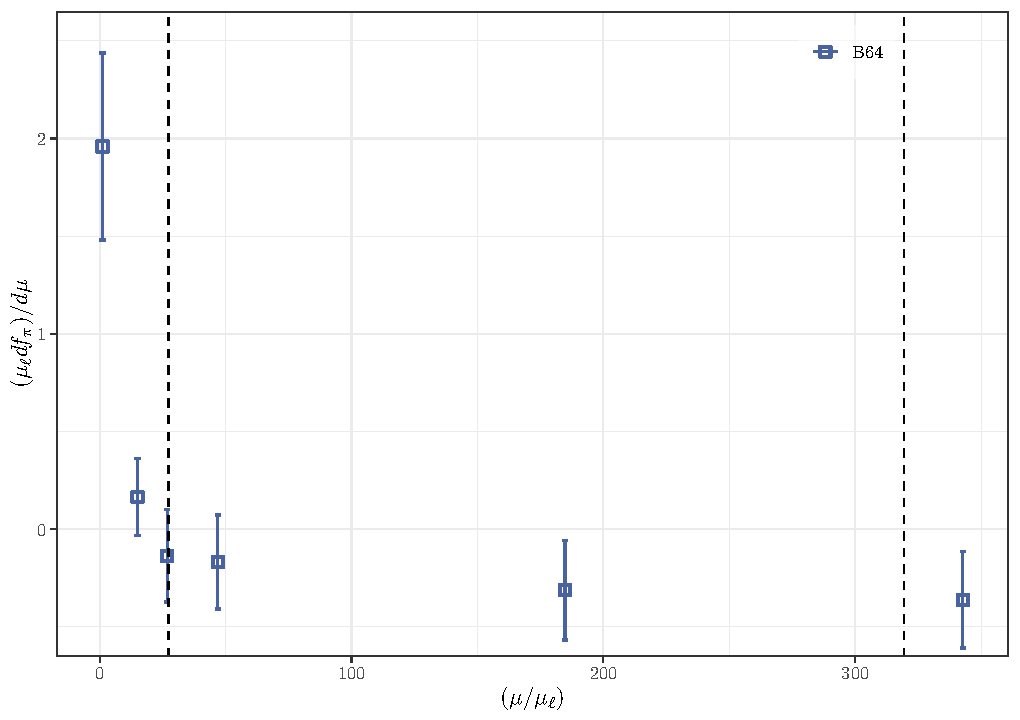
\includegraphics[scale=0.5]{plots/der_fpi_B64.pdf}
      \end{center}
  \end{itemize}
\end{frame}

\begin{frame}
  \begin{itemize}
    \item renormalized quantity $\mu_\ell  \frac{\partial f_\pi }{\partial\mu}$ computed for more lattice spacing
  \end{itemize}
  \begin{columns}
    \begin{column}{0.5\textwidth}
      \begin{itemize}
        \item fit $\mu_\ell  \frac{\partial f_\pi }{\partial\mu} = P_0\frac{1}{\mu} +P_1\frac{1}{\mu^2}+P_2\frac{1}{\mu^2}$
        \item $\chi^2/d.o.f=2$
      \end{itemize}
    \end{column}
    \begin{column}{0.5\textwidth}
      \begin{itemize}
        \item<2-> Rescale errors such $\chi^2/d.o.f=1$
        \item<2-> Equivalent of rescaling the fit parameters error $\tilde P = P \sqrt{\chi^2/d.o.f}$
      \end{itemize}
    \end{column}
  \end{columns}

  \begin{columns}
    \begin{column}{0.5\textwidth}
      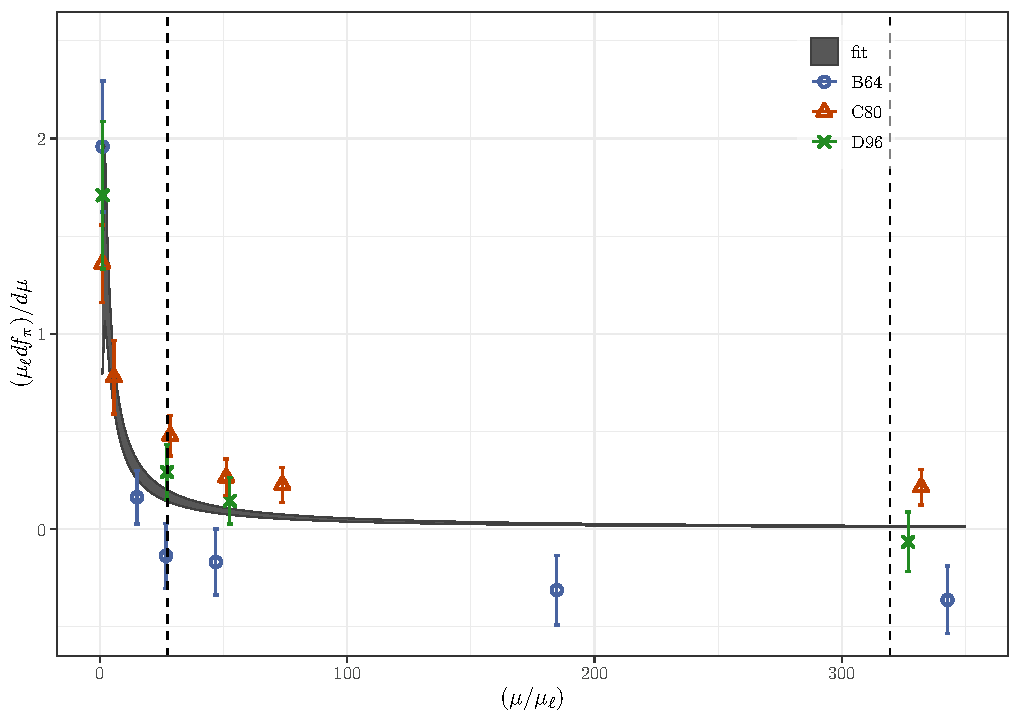
\includegraphics[scale=0.5]{plots/der_fpi_fit.pdf}
    \end{column}
    \begin{column}{0.5\textwidth}
      \uncover<2->{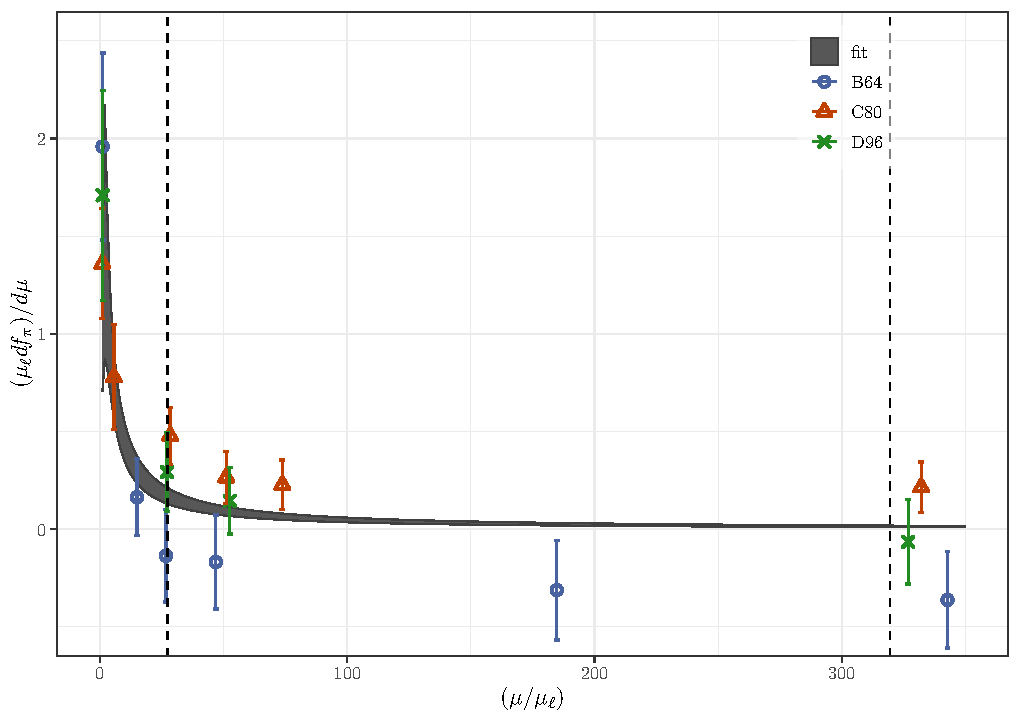
\includegraphics[scale=0.5]{plots/der_fpi_fit_chi2d1.pdf}}
    \end{column}
  \end{columns}
\end{frame}

\begin{frame}
  \begin{columns}
    \begin{column}{0.5\textwidth}
      \begin{itemize}
        \item Same procedure for $M_\pi$\\
              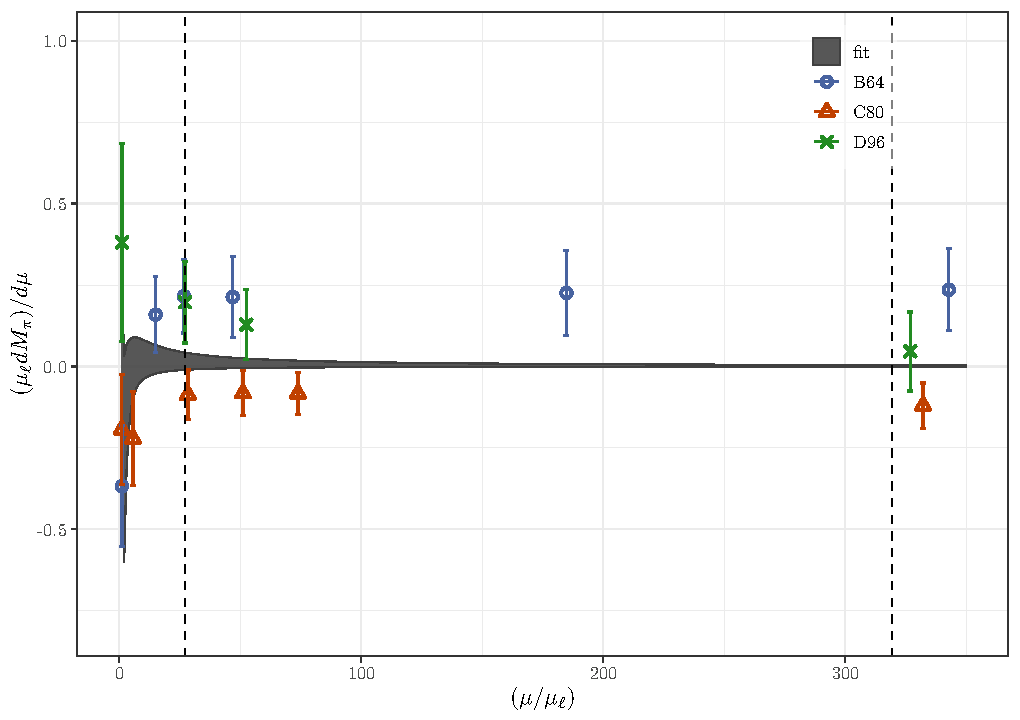
\includegraphics[scale=0.5]{plots/der_Mpi_fit_chi2d1.pdf}
      \end{itemize}
    \end{column}
    \begin{column}{0.5\textwidth}
      \begin{tabular}{c|c|c|c|c}
        ensemble & $\Delta_s f_\pi / \sigma_{f_\pi}$ & $\Delta_c f_\pi / \sigma_{f_\pi}$ \\
        B64      & 0.69                              & 0.36                              \\
        C80      & -1.2                              & 0.67                              \\
        D96      & 0.46                              & 0.89                              \\
        E112     & 0.45                              & -0.27
      \end{tabular}
      \vspace*{1cm}\,
      \begin{tabular}{c|c|c|c|c}
        ensemble & $\Delta_s M_\pi / \sigma_{M_\pi}$ & $\Delta_c M_\pi / \sigma_{M_\pi}$ \\
        B64      & 0.10                              & 0.06                              \\
        C80      & -0.16                             & 0.11                              \\
        D96      & 0.05                              & 0.13                              \\
        E112     & 0.05                              & -0.04
      \end{tabular}
    \end{column}
  \end{columns}
\end{frame}

\begin{frame}{insignificance of sea mass mistunings on $M_K$ and $M_{D_s}$}
  Same procedure for $M_K$ and $M_{D_s}$, but slightly different implementation: 
  \begin{itemize}
  \item constant fit between the three (available) ensembles for $\ell$- and $s$-contributions
  \item fit $\mu_\ell  \frac{\partial M }{\partial\mu} = P_0\frac{1}{\mu^2}+P_1\frac{1}{\mu^2}$ in the range $\mu_s\le\mu\le\mu_c$ to evaluate the $c$-contribution
  \item all the errors rescaled with $\sqrt{\chi^2_\mathrm{red}}$ when $\chi^2_\mathrm{red}>1$ 
  \end{itemize}
\begin{columns}
    \begin{column}{0.5\textwidth}
       \begin{center}
       % Tabella per m_l
       \begin{tabular}{l|c|c}
       Ensemble
       & $\Delta_{\ell}M_{K}$ [MeV]
       & $\Delta_{\ell}M_{K}/\sigma_{M_{K}}$ \\
       B64  & $0.0275(245)$ & $0.0773$ \\
       C80  & $0.0080(71)$  & $0.0147$ \\
       D96  & $0.0327(291)$ & $0.0457$ \\
       \end{tabular}
       \vspace*{0.2cm}\,
       \\
       % Tabella per m_s
       \begin{tabular}{l|c|c}
       Ensemble
       & $\Delta_{s}M_{K}$ [MeV]
       & $\Delta_{s}M_{K}/\sigma_{M_{K}}$ \\
       B64  & $0.0689(543)$  & $0.193$ \\
       C80  & $-0.111(87)$   & $-0.203$ \\
       D96  & $0.0361(284)$  & $0.0504$ \\
       \end{tabular}
       \vspace*{0.2cm}\,
       \\
       % Tabella per m_c
       \begin{tabular}{l|c|c}
       Ensemble
       & $\Delta_{c}M_{K}$ [MeV]
       & $\Delta_{c}M_{K}/\sigma_{M_{K}}$ \\
       B64  & $0.0071(221)$  & $0.0200$ \\
       C80  & $0.0097(303)$  & $0.0178$ \\
       D96  & $-0.0111(346)$ & $-0.0155$ \\
       \end{tabular}
       \end{center}
    \end{column}
    \begin{column}{0.5\textwidth}
    \begin{center}
    % Tabella per m_l
    \begin{tabular}{l|c|c}
    Ensemble
    & $\Delta_{\ell}M_{D_s}$ [MeV]
    & $\Delta_{\ell}M_{D_s}/\sigma_{M_{D_s}}$ \\
    B64  & $0.0340(333)$ & $0.02766$ \\
    C80  & $0.0099(97)$  & $0.00495$ \\
    D96  & $0.0404(395)$ & $0.01473$ \\
    \end{tabular}
    \vspace*{0.2cm}\,
    \\
    % Tabella per m_s
    \centering
    \begin{tabular}{l|c|c}
    Ensemble
    & $\Delta_{s}M_{D_s}$ [MeV]
    & $\Delta_{s}M_{D_s}/\sigma_{M_{D_s}}$ \\
    B64  & $0.288(125)$  & $0.234$ \\
    C80  & $-0.463(200)$ & $-0.231$ \\
    D96  & $0.151(65)$   & $0.05499$ \\
    \end{tabular}
    \vspace*{0.2cm}\,
    \\
    % Tabella per m_c
    \centering
    \begin{tabular}{l|c|c}
    Ensemble
    & $\Delta_{c}M_{D_s}$ [MeV]
    & $\Delta_{c}M_{D_s}/\sigma_{M_{D_s}}$ \\
    B64  & $0.0642(603)$  & $0.05215$ \\
    C80  & $0.0879(83)$   & $0.0439$ \\
    D96  & $-0.100(94)$   & $-0.0366$ \\
    \end{tabular}
    \end{center}
    \end{column}
  \end{columns}
\vspace*{0.1cm}\,
\begin{itemize}
    \item As shown, all the contributions are negligible wrt the errors on the meson masses (the sum of all the contributions is negligible as well).
\end{itemize}
\end{frame}

\begin{frame}
    
   \begin{columns}
       \begin{column}{0.5\textwidth}
        {\small $$\mu_\ell \frac{\partial M_{K}}{\partial \mu_\ell} = -0.35(31); \qquad\frac{\chi^2}{\rm d.o.f}= 0.1$$}
        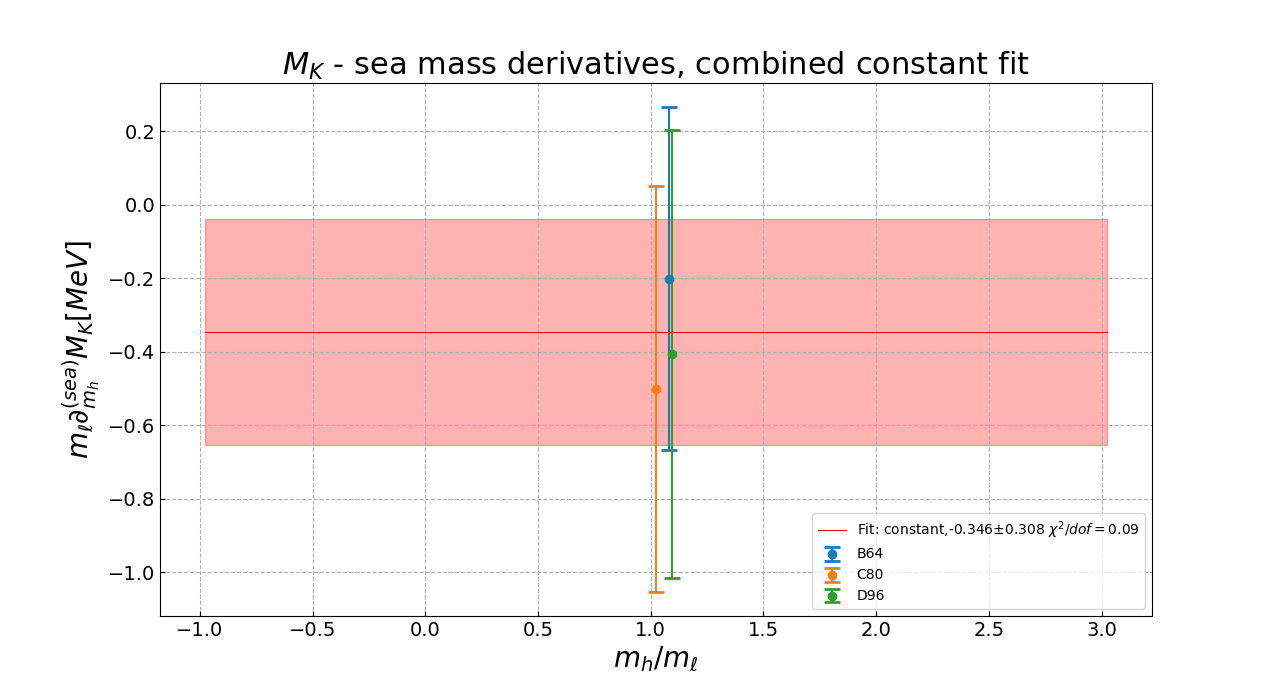
\includegraphics[trim=0cm 0.5cm 0cm 1.3cm, clip,width=\textwidth]{plots/const_fit_MK_der_ml.png}
        \vspace*{-0.8cm} \,\\
        {\small $$\mu_\ell \frac{\partial M_{K}}{\partial \mu_s} = -0.11(9); \qquad\frac{\chi^2}{\rm d.o.f}= 1.3$$}
        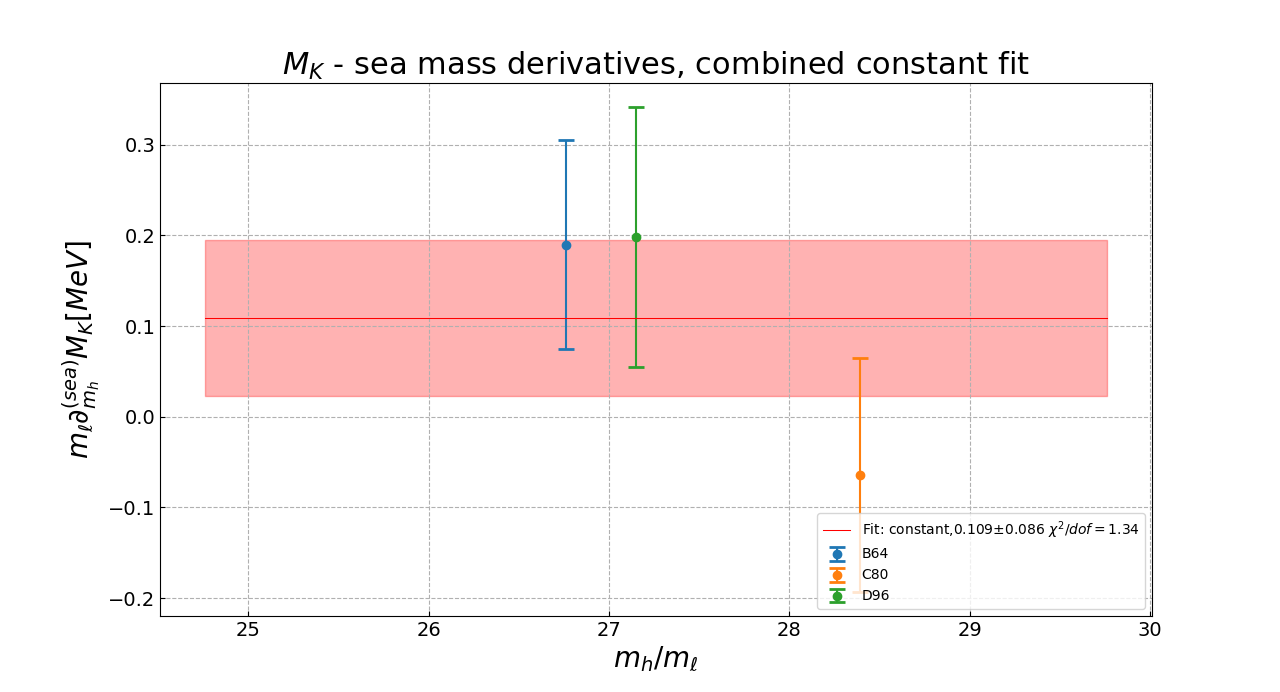
\includegraphics[trim=0cm 0.5cm 0cm 1.3cm, clip,width=\textwidth]{plots/const_fit_MK_der_ms.png}
       \end{column}
       \begin{column}{0.5\textwidth}
        {\small $$\mu_\ell \frac{\partial M_{D_s}}{\partial \mu_\ell} = -0.43(42); \qquad\frac{\chi^2}{\rm d.o.f}= 0.1$$}
        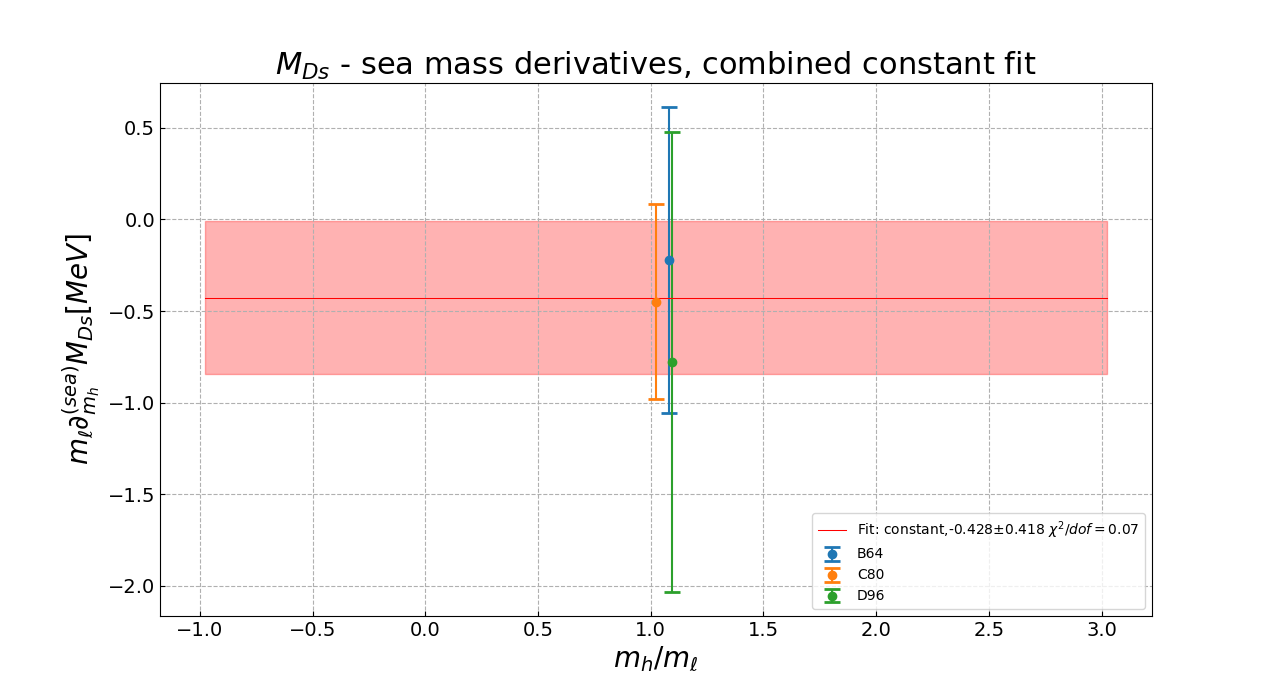
\includegraphics[trim=0cm 0.5cm 0cm 1.3cm, clip,width=\textwidth]{plots/const_fit_MD_der_ml.png}
        \vspace*{-0.8cm} \,\\
        {\small $$\mu_\ell \frac{\partial M_{D_s}}{\partial \mu_s} = -0.46(20); \qquad\frac{\chi^2}{\rm d.o.f}= 3.19$$}
        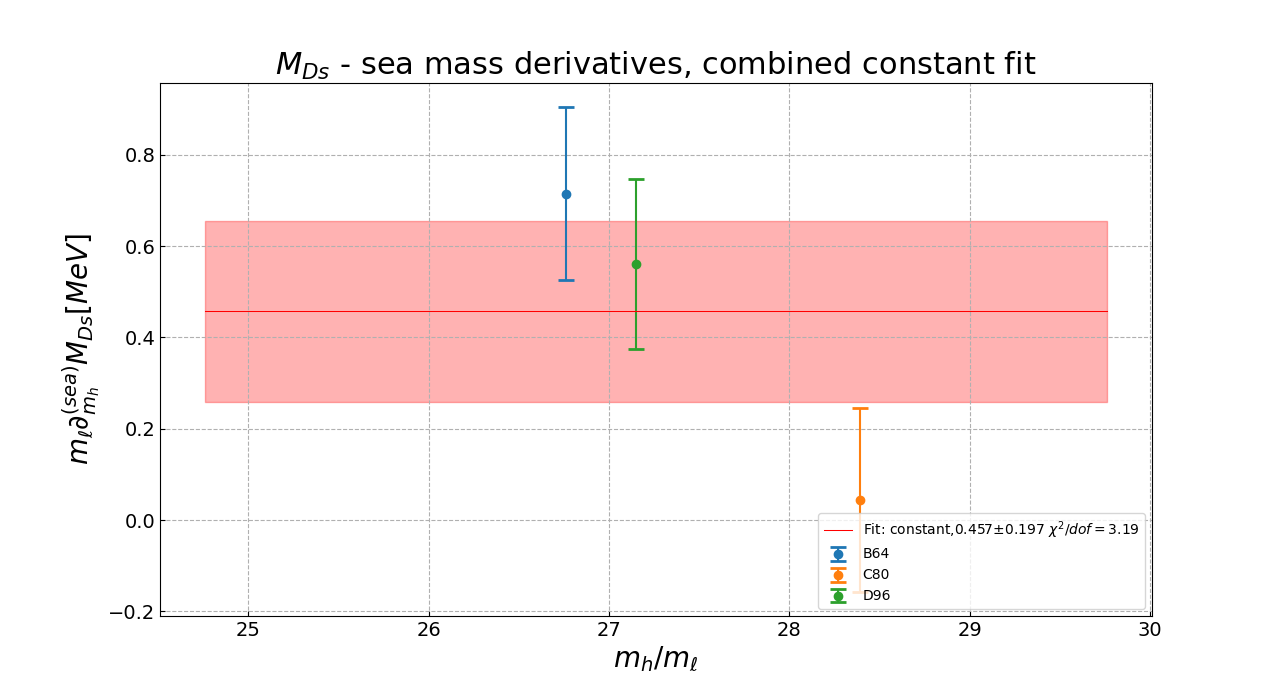
\includegraphics[trim=0cm 0.5cm 0cm 1.3cm, clip,width=\textwidth]{plots/const_fit_MD_der_ms.png}
       \end{column}
   \end{columns}
\end{frame}

\begin{frame}
   \begin{columns}
       \begin{column}{0.5\textwidth}
        {\small $$\mu_\ell \frac{\partial M_K}{\partial \mu_c} = -0.0016(49); \qquad\frac{\chi^2}{\rm d.o.f}= 2.0$$}
        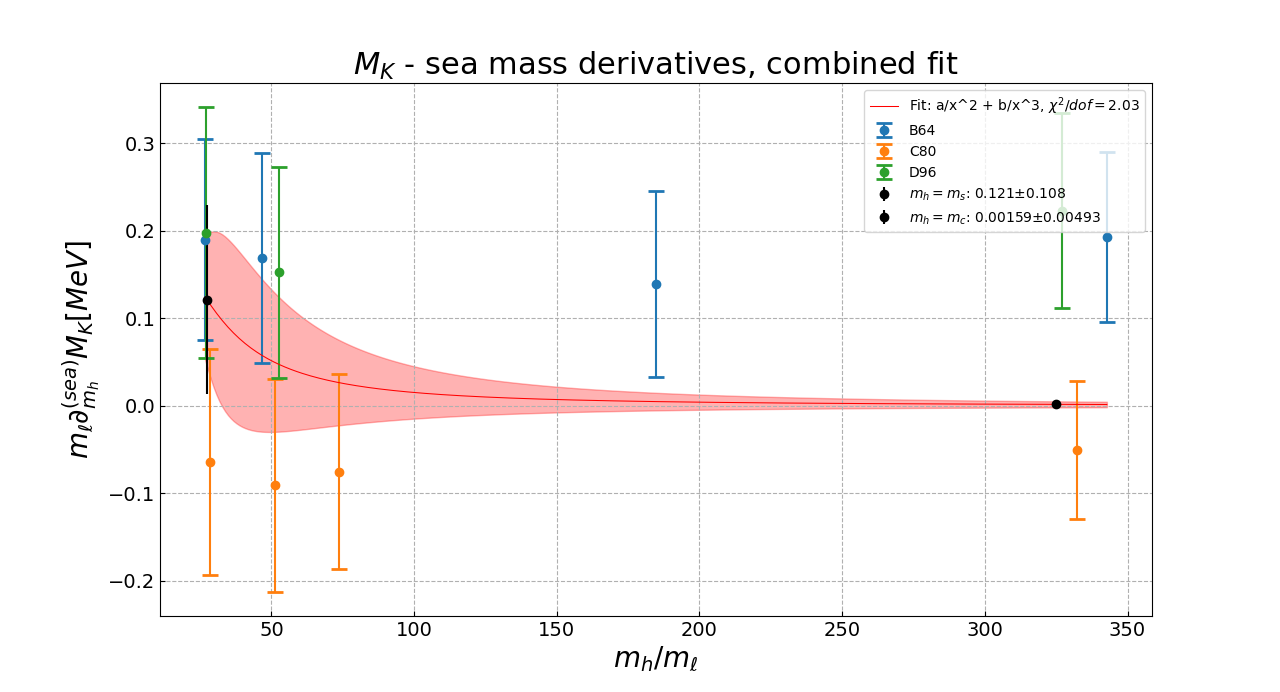
\includegraphics[trim=0cm 0.5cm 0cm 1.3cm, clip,width=\textwidth]{plots/deco_fit_MK_der_mc.png}
       \end{column}
       \begin{column}{0.5\textwidth}
        {\small $$\mu_\ell \frac{\partial M_{D_s}}{\partial \mu_c} = -0.014(13); \qquad\frac{\chi^2}{\rm d.o.f}= 5.3$$}
        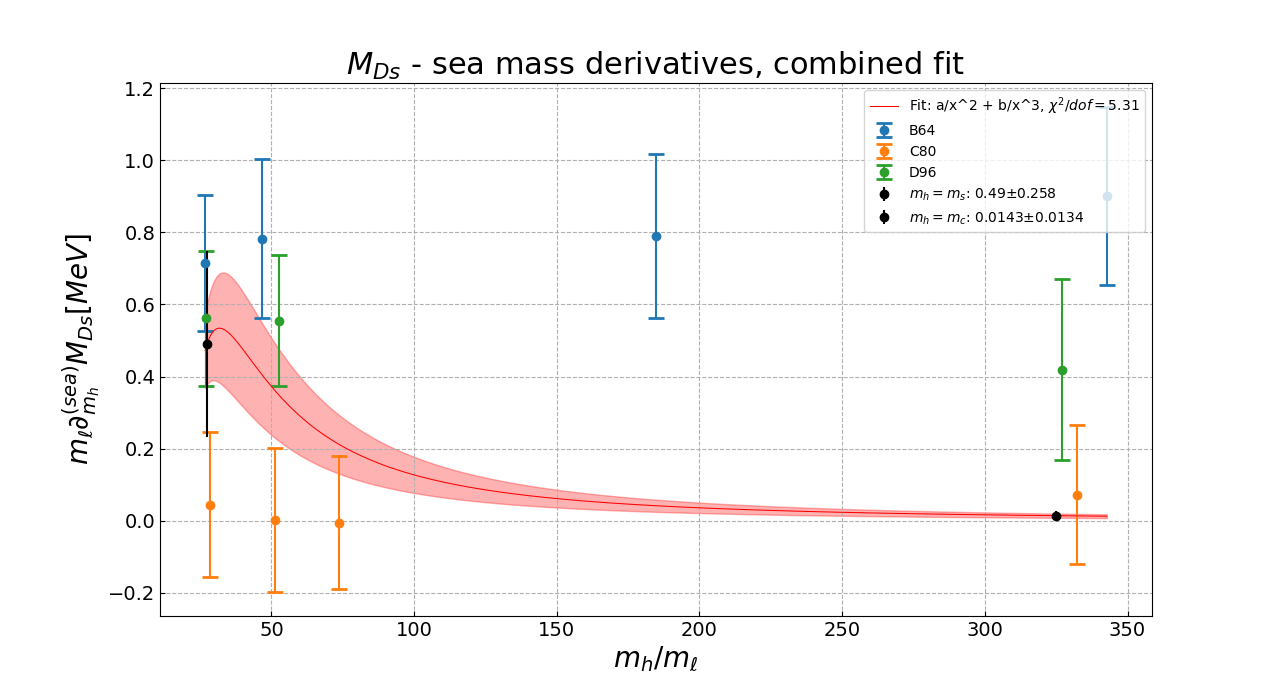
\includegraphics[trim=0cm 0.5cm 0cm 1.3cm, clip,width=\textwidth]{plots/deco_fit_MD_der_mc.png}
       \end{column}
   \end{columns}
   These results are obtained using the fit ansatz:
   \[
   \mu_\ell  \frac{\partial M }{\partial\mu} = P_0\frac{1}{\mu^2}+P_1\frac{1}{\mu^2},
   \]
   and are those used to produce the tables above. For comparison, we also tried to fit with the same ansatz used for $M_\pi$ and $f_\pi$ and $f_\pi$. Plots and discussion in the next slide.
\end{frame}
\begin{frame}
   \begin{columns}
       \begin{column}{0.5\textwidth}
        {\small $$\mu_\ell \frac{\partial M_K}{\partial \mu_c} = -0.0077(80); \qquad\frac{\chi^2}{\rm d.o.f}= 1.44$$}
        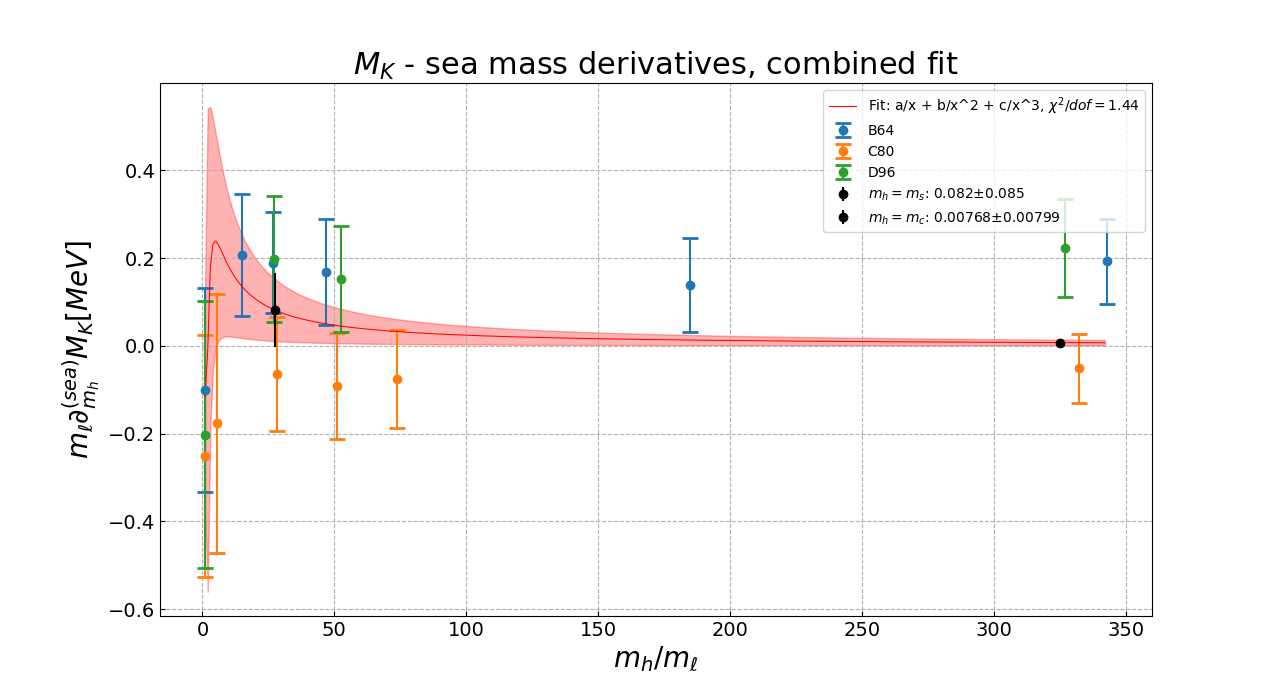
\includegraphics[trim=0cm 0.5cm 0cm 1.3cm, clip,width=\textwidth]{plots/deco_fit_MK_der_mc_lin_term.png}
       \end{column}
       \begin{column}{0.5\textwidth}
        {\small $$\mu_\ell \frac{\partial M_{D_s}}{\partial \mu_c} = 0.034(18); \qquad\frac{\chi^2}{\rm d.o.f}= 3.78$$}
        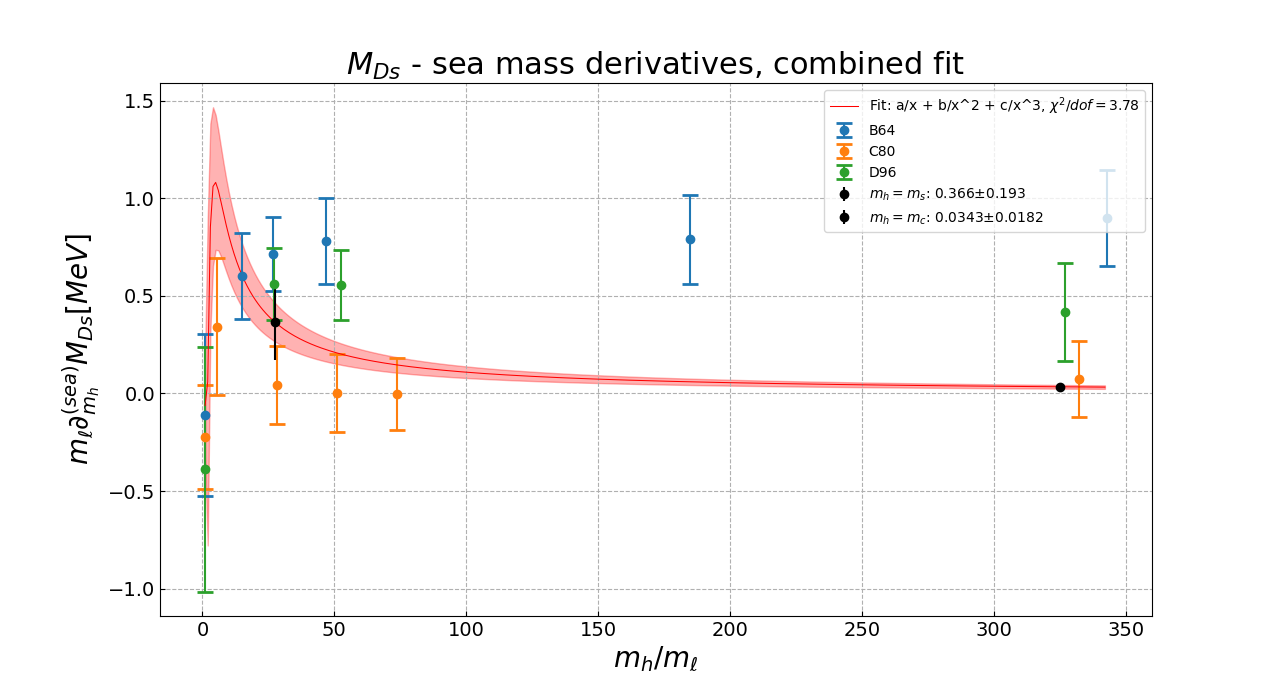
\includegraphics[trim=0cm 0.5cm 0cm 1.3cm, clip,width=\textwidth]{plots/deco_fit_MD_der_mc_lin_term.png}
       \end{column}
   \end{columns}
   
   These results are obtained using the fit ansatz:
   \[
   \mu_\ell  \frac{\partial M }{\partial\mu} = P_0\frac{1}{\mu}+P_1\frac{1}{\mu^2}+P_2\frac{1}{\mu^3}.
   \]
   We obtain similar results for the derivative w.r.t $\mu_s$; for the derivatives w.r.t. $\mu_c$, these results are, respectively, 5 times and 3 times larger for $M_K$ and $M_{D_s}$. Even so, almost all the shifts would be negligible w.r.t. the errors on the meson masses. The only exception being the shift on $M_K$ in the \texttt{B64} ensemble: $\Delta_{\ell+s+c}M_K\simeq0.4\sigma_{M_K}$.
\end{frame}
\begin{frame}
  \begin{itemize}
    \item Unitary analysis
          \begin{align*}
            aF_{\pi}(\xi_{\pi}, \beta) & =  a\overline{F}_{\pi}(\beta) \cdot \left\{1-2\xi_{\pi}\log(\xi_{\pi}/\xi_{\pi}^{\rm iso})+ [P+P_{disc} (aF_\pi(\xi_{\pi},\beta))^2] (\xi_{\pi}-\xi^{\rm iso}_{\pi})\right\}
          \end{align*}
          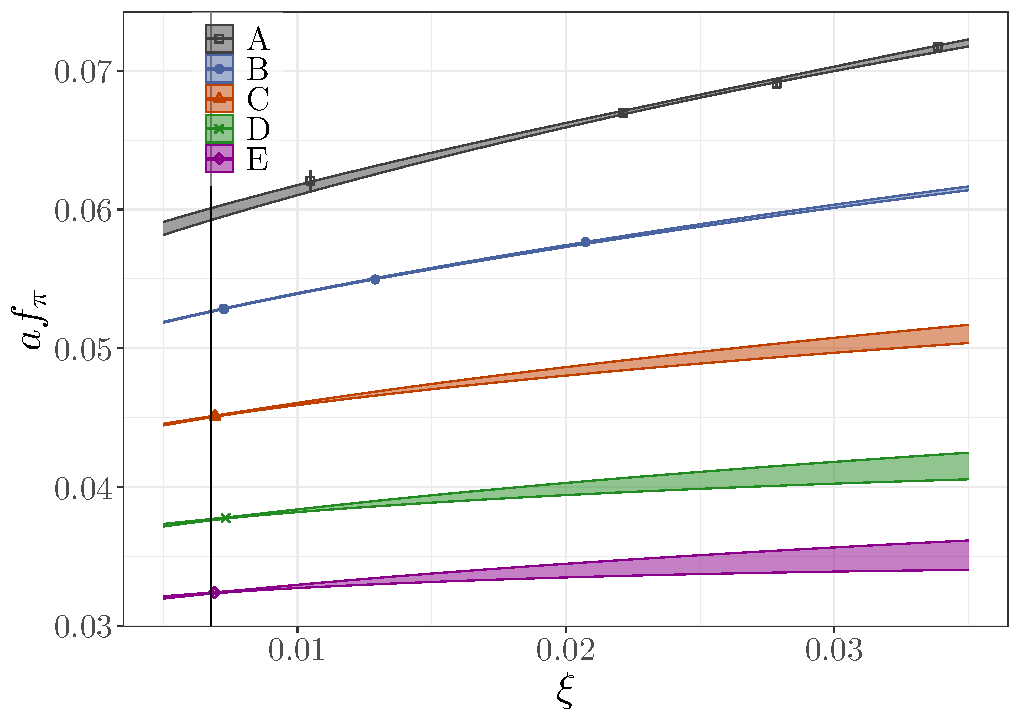
\includegraphics[scale=0.5]{plots/fpi_rew}
          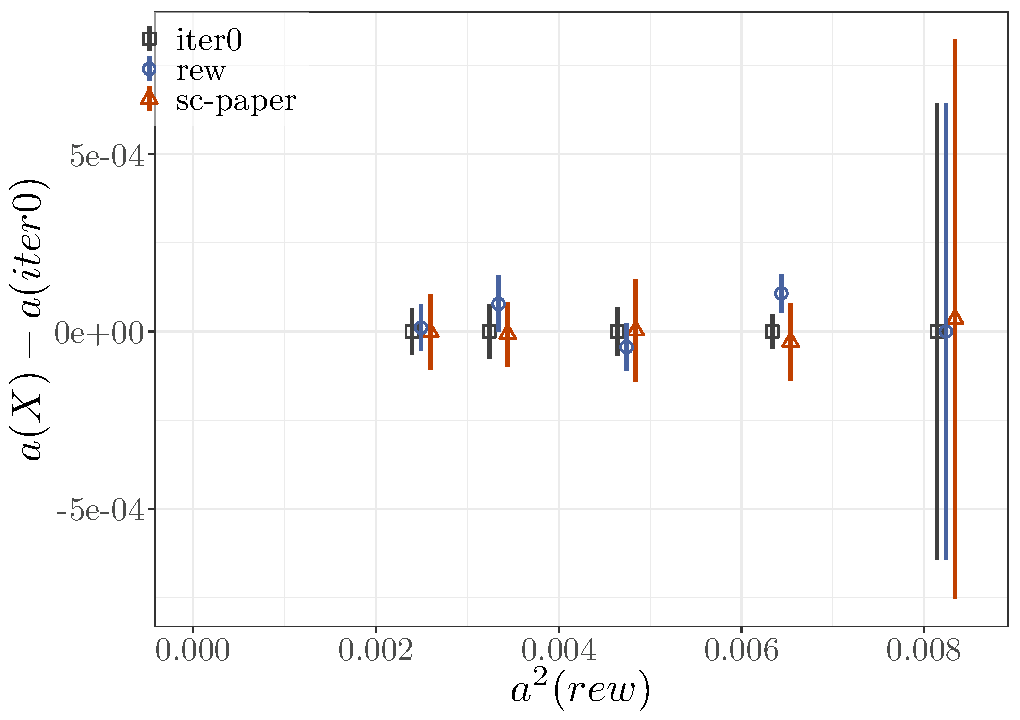
\includegraphics[scale=0.5]{plots/scaling_a}
  \end{itemize}
\end{frame}

\begin{frame}
  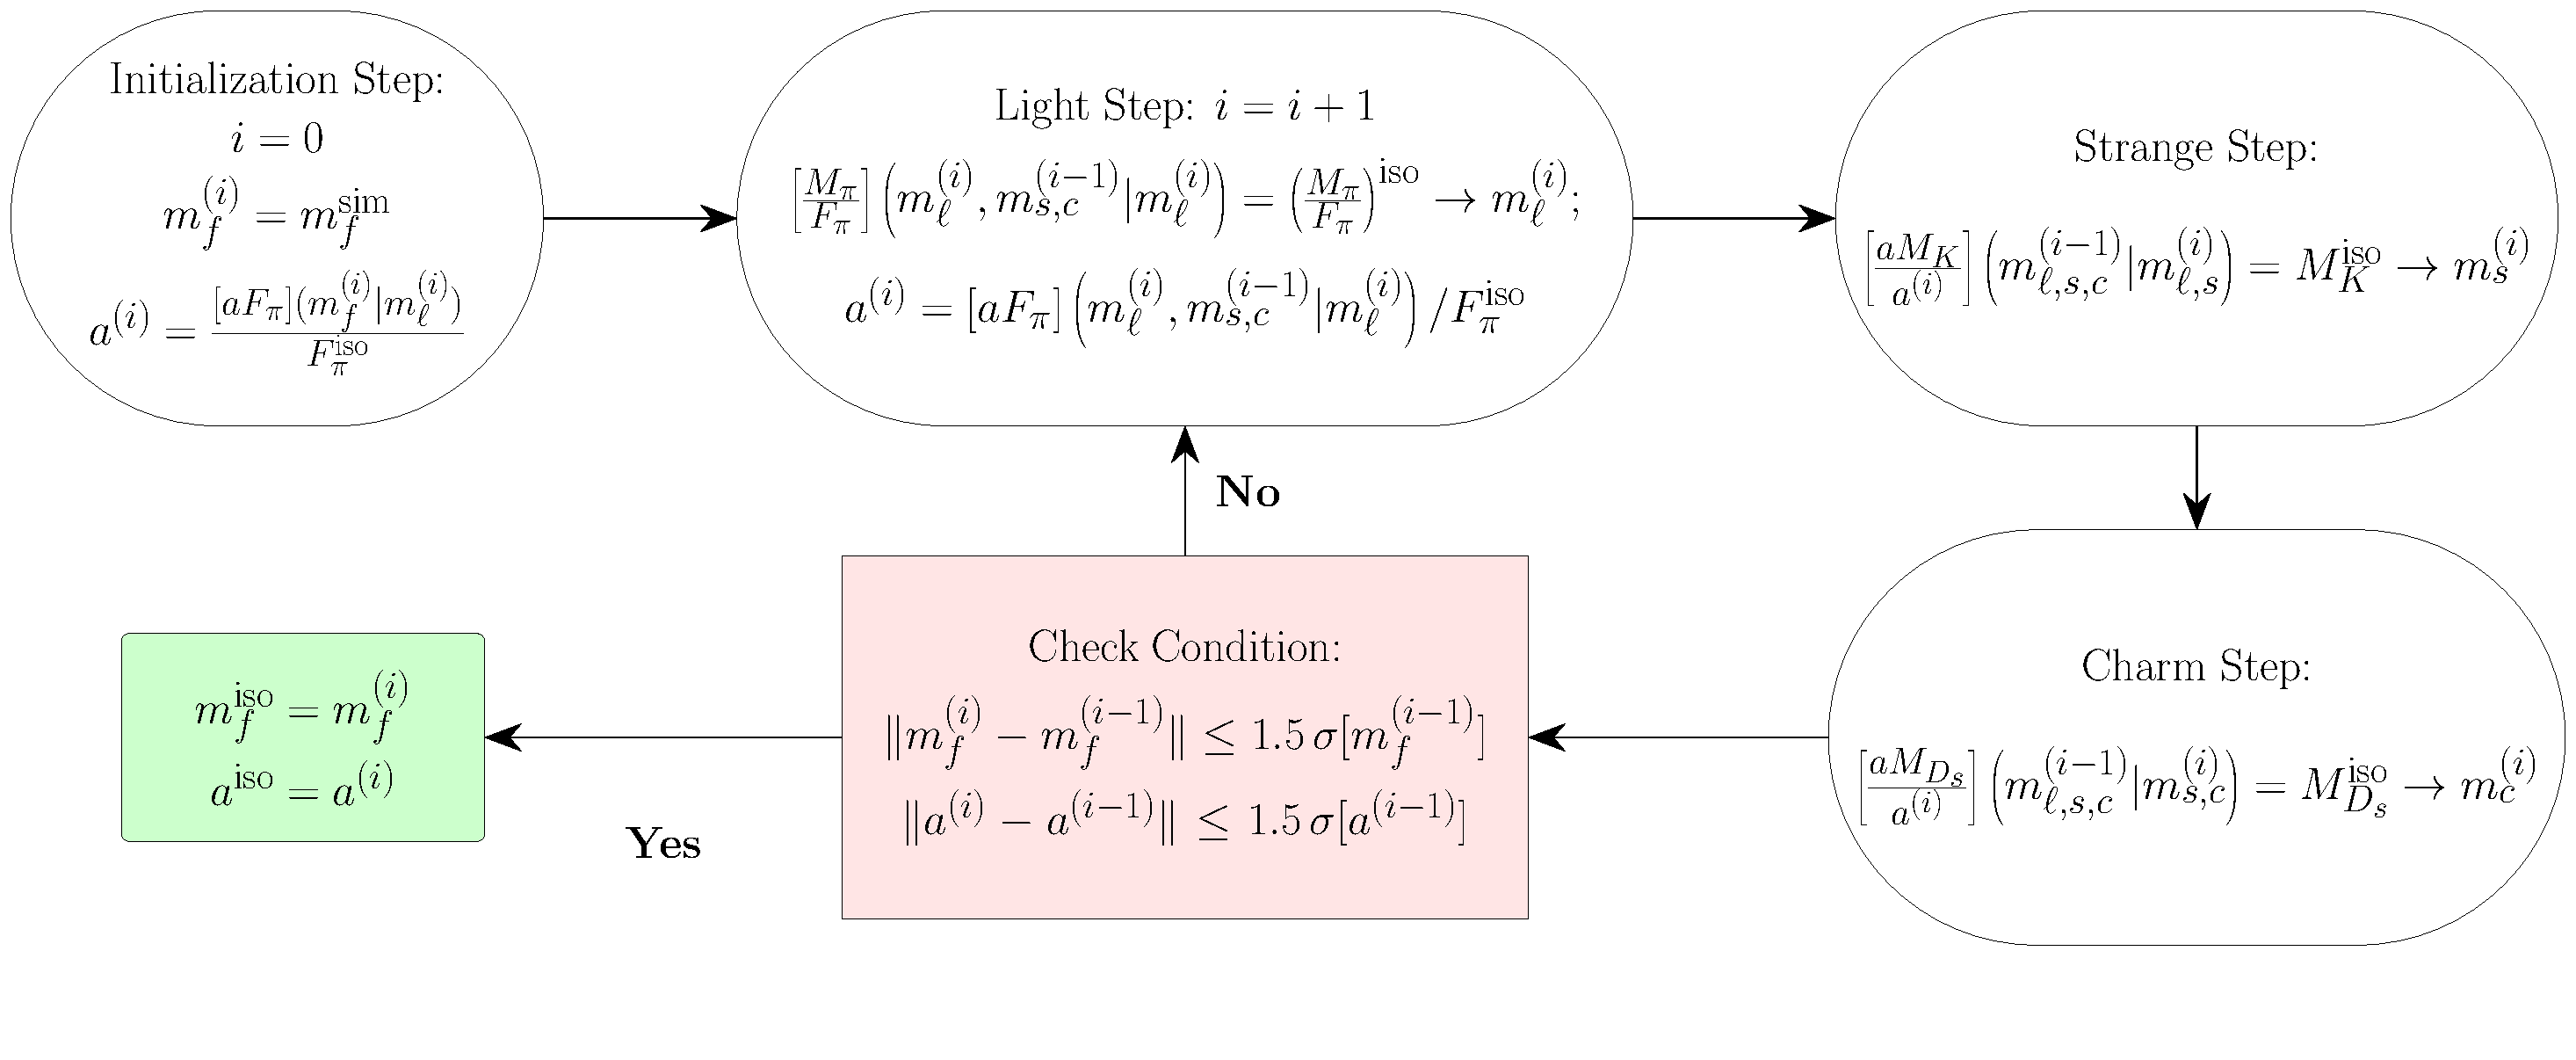
\includegraphics[scale=0.35]{lat_algo.pdf} \\
  {\huge{\color{green!40}$\checkmark$}} Check passed
\end{frame}

\begin{frame}
  \begin{itemize}
    \item Unitary analysis
          \begin{align*}
            am_{\ell}(\xi_{\pi},\beta) & = a\overline{m}_{\ell}(\beta) \frac{\xi_{\pi}}{\xi_{\pi}^{\rm iso}} \cdot \left\{ 1 + 5\xi_{\pi}\log(\xi_{\pi}/\xi_{\pi}^{\rm iso}) + (B+a^2B_{disc})(\xi_{\pi} -\xi_{\pi}^{\rm iso}) \right\}^{-1}
          \end{align*}
          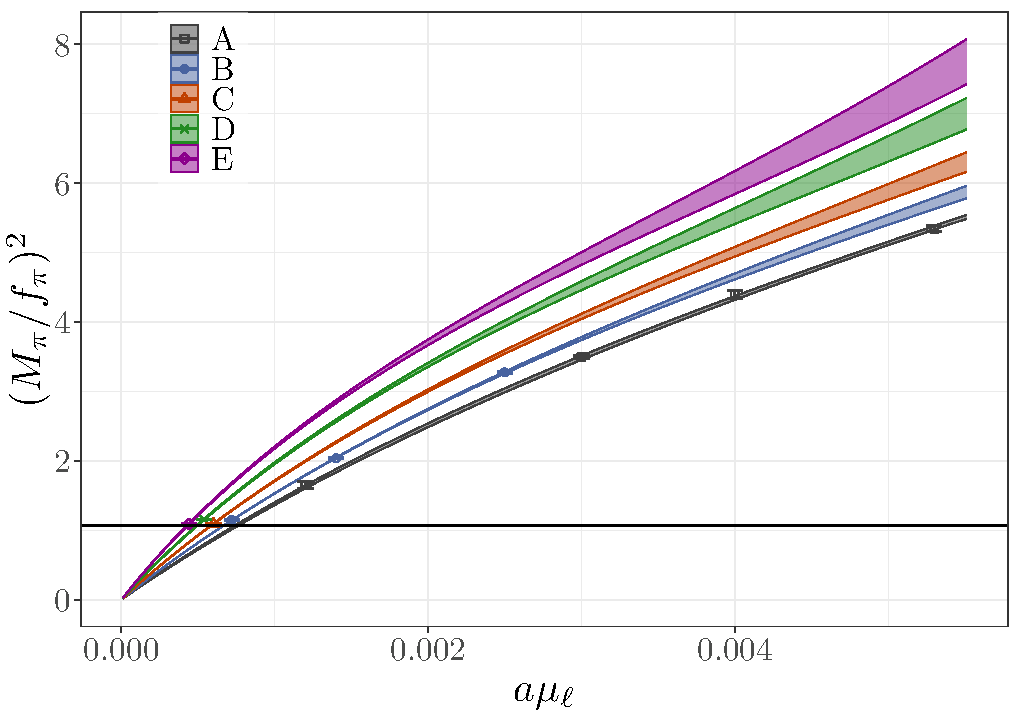
\includegraphics[scale=0.5]{plots/Mpi_rew}
          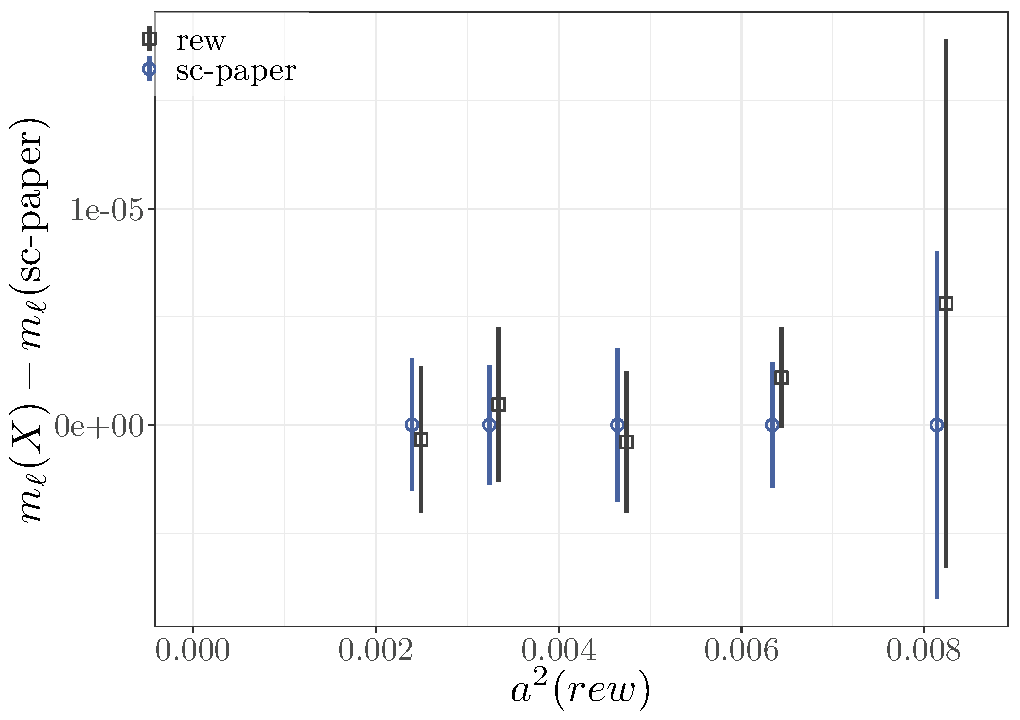
\includegraphics[scale=0.5]{plots/ml_scaling}
  \end{itemize}
\end{frame}

\begin{frame}
  \begin{itemize}
    \item scale setting trough $w_0$ BMW ($\Omega$)
    \item<2-> in progress
  \end{itemize}
\end{frame}

\begin{frame}{Sea mass mistunings on $a_\mu^\mathrm{HVP}(\ell)^\mathrm{conn}$}
    \begin{itemize}
        \item the derivative of $a_\mu^\mathrm{HVP}(\ell)^\mathrm{conn}$ is given by
        \[
        \partial^\mathrm{sea}_{\mu_q}a_\mu^\mathrm{HVP}(\ell)^\mathrm{conn} = \int_0^\infty dt \, t^2 \, K(t\ m_\mu) \,\, \partial^\mathrm{sea}_{\mu_q}<V_k(\ell)\, V_k(\ell)>^\mathrm{conn}
        \]
        \\ \
        \item $\partial^\mathrm{sea}_{\mu_q}<V_k(\ell)\, V_k(\ell)>^\mathrm{conn}$ is computed using the reweighting factors;\\ \
        \item the time integration must be performed carefully, to avoid putting in too much noise;\\ \
        \item then, the renormalized quantity $\mu_\ell\frac{\partial a_\mu^\mathrm{HVP}(\ell)^\mathrm{conn}}{\partial \mu}$ can be compared among different ensembles (as before);\\ \
        \item we use results from both the TM and OS discretizations to increase statistics (taking care of the correlations);\\ \
        \item we perform a constant fit of the derivatives for the $\ell$ and $s$ contributions, and a "decoupling-inspired" fit for the $c$ contribution.
    \end{itemize}
\end{frame}
\begin{frame}
    For the $\ell$-contribution, we integrate up to the t-cut selected for $a_\mu^\mathrm{HVP}(\ell)^\mathrm{SIM}$ with the ETM bounding method.
    \begin{columns}
    \begin{column}{0.5\textwidth}
     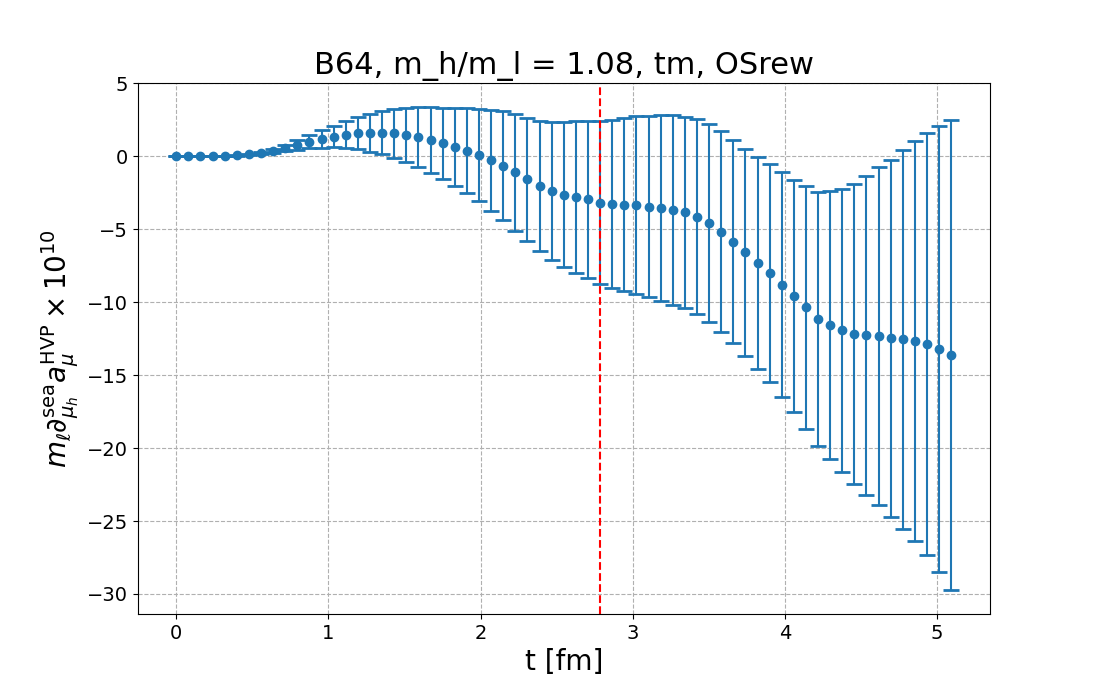
\includegraphics[trim=0cm 0.3cm 0cm 1.2cm, clip,width=\textwidth]{plots/der_mq_sea_lore/amu_B64_tm_der_001ml.png}
     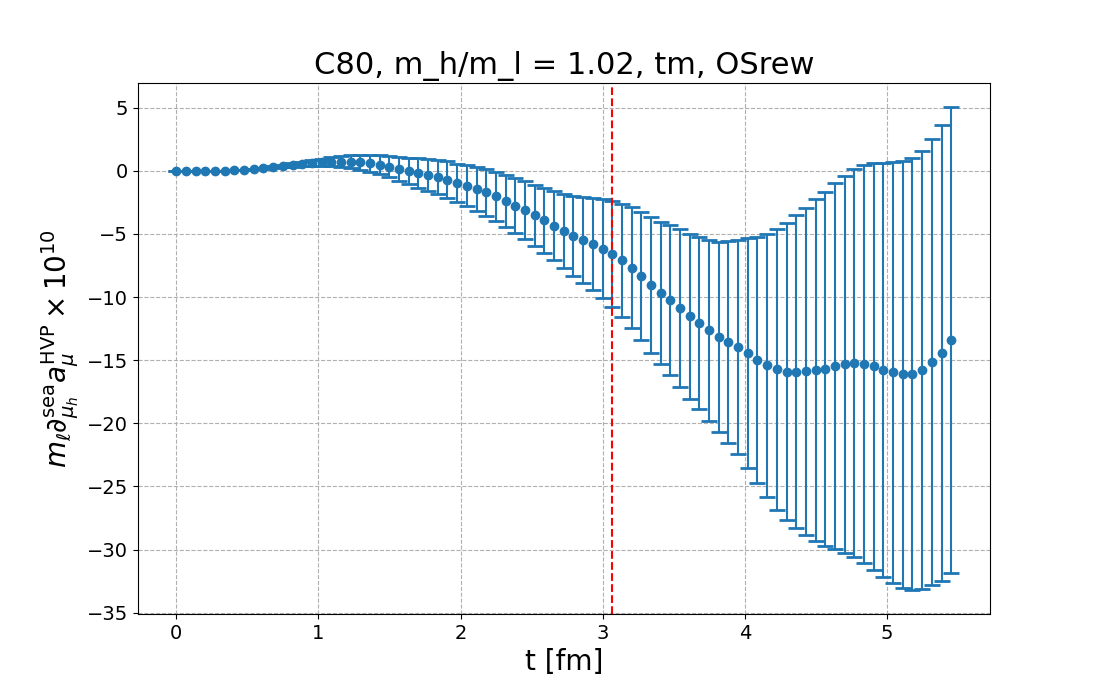
\includegraphics[trim=0cm 0.3cm 0cm 1.2cm, clip,width=\textwidth]{plots/der_mq_sea_lore/amu_C80_tm_der_001ml.png}
    \end{column}
    \begin{column}{0.5\textwidth}
     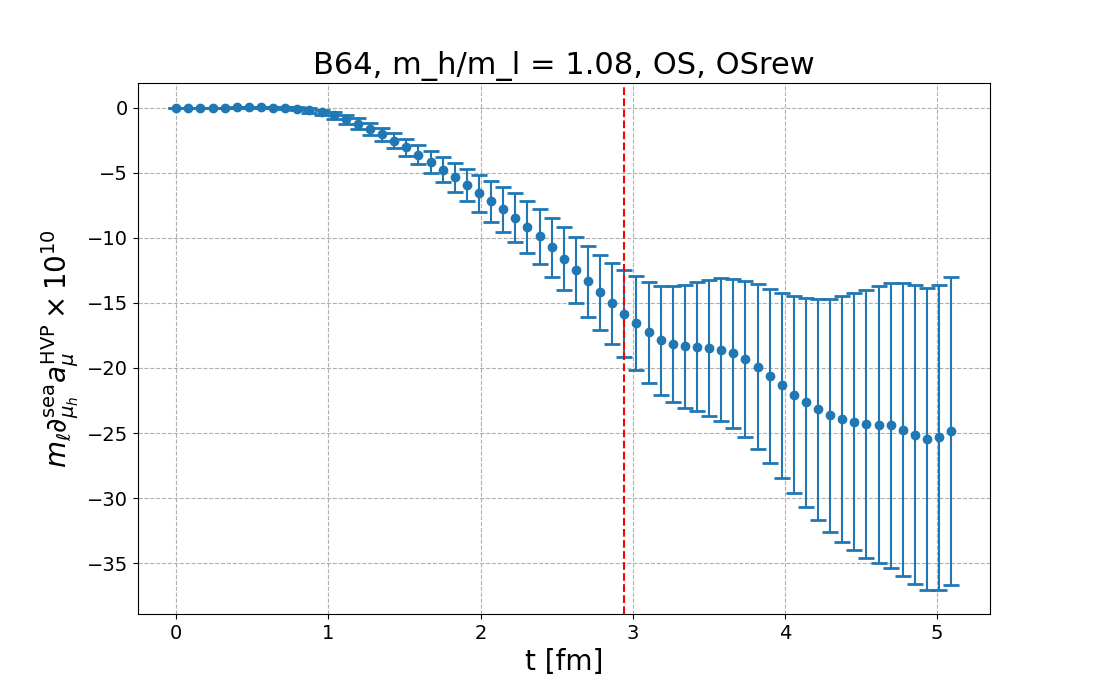
\includegraphics[trim=0cm 0.3cm 0cm 1.2cm, clip,width=\textwidth]{plots/der_mq_sea_lore/amu_B64_OS_der_001ml.png}
     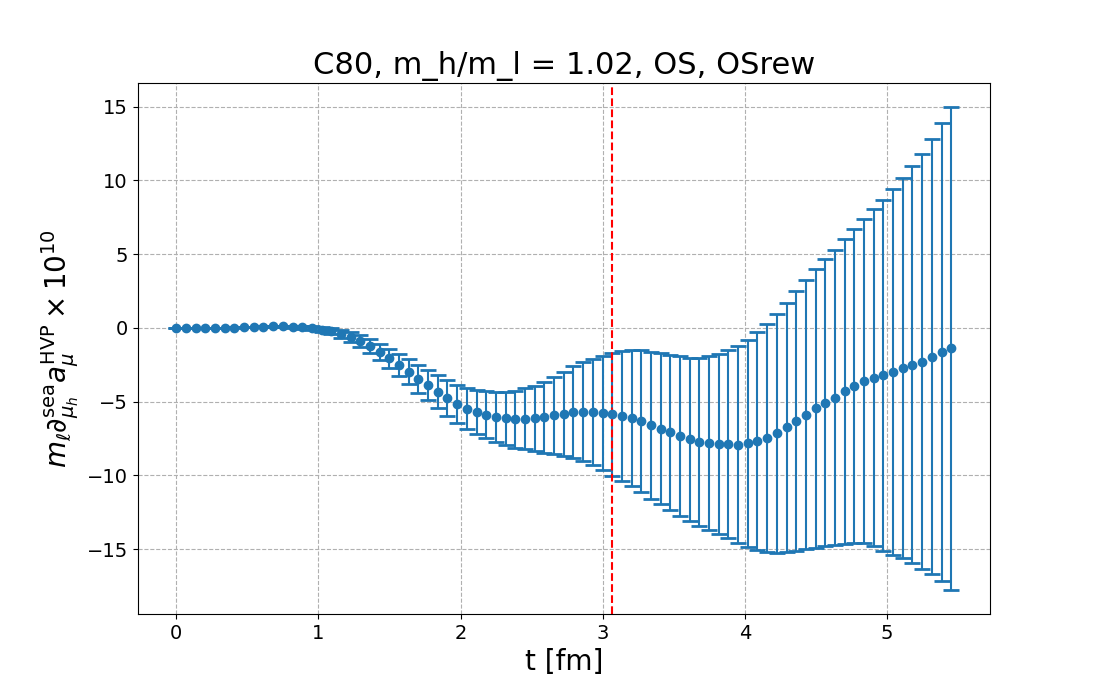
\includegraphics[trim=0cm 0.3cm 0cm 1.2cm, clip,width=\textwidth]{plots/der_mq_sea_lore/amu_C80_OS_der_001ml.png}
    \end{column}
   \end{columns}
\end{frame}
\begin{frame}
    For the $\ell$-contribution, we integrate up to the t-cut selected for $a_\mu^\mathrm{HVP}(\ell)^\mathrm{SIM}$ with the ETM bounding method.\vfill \,

    \

    \
    
    \
    
    \begin{columns}
    \begin{column}{0.5\textwidth}
     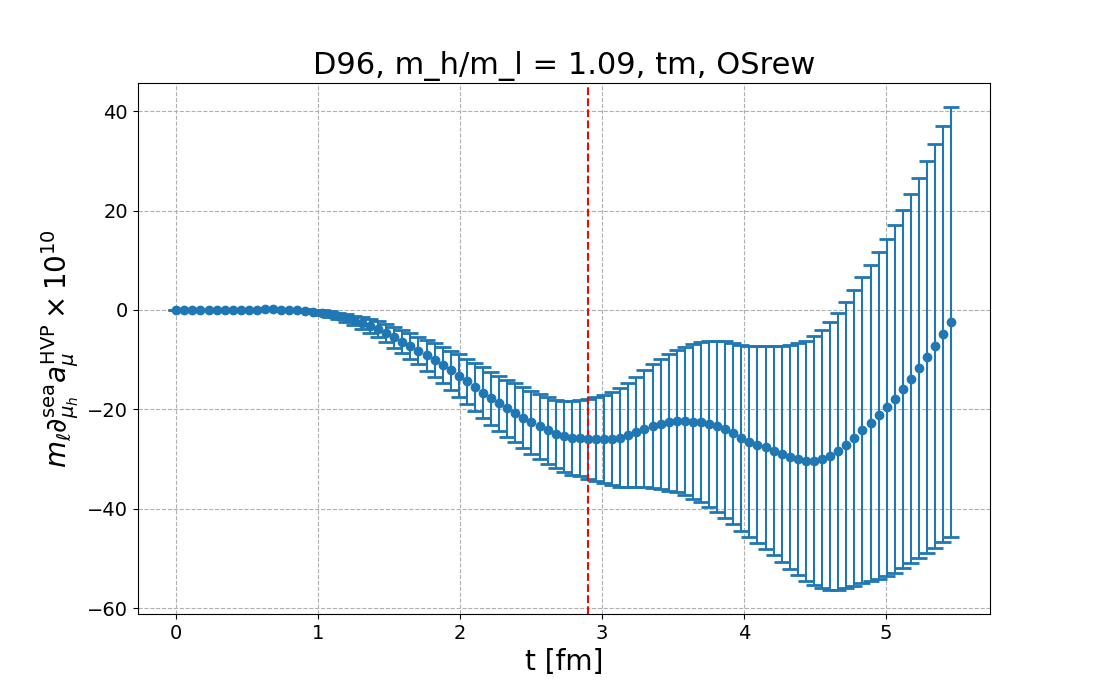
\includegraphics[trim=0cm 0.3cm 0cm 1.2cm, clip,width=\textwidth]{plots/der_mq_sea_lore/amu_D96_tm_der_001ml.png}
    \end{column}
    \begin{column}{0.5\textwidth}
     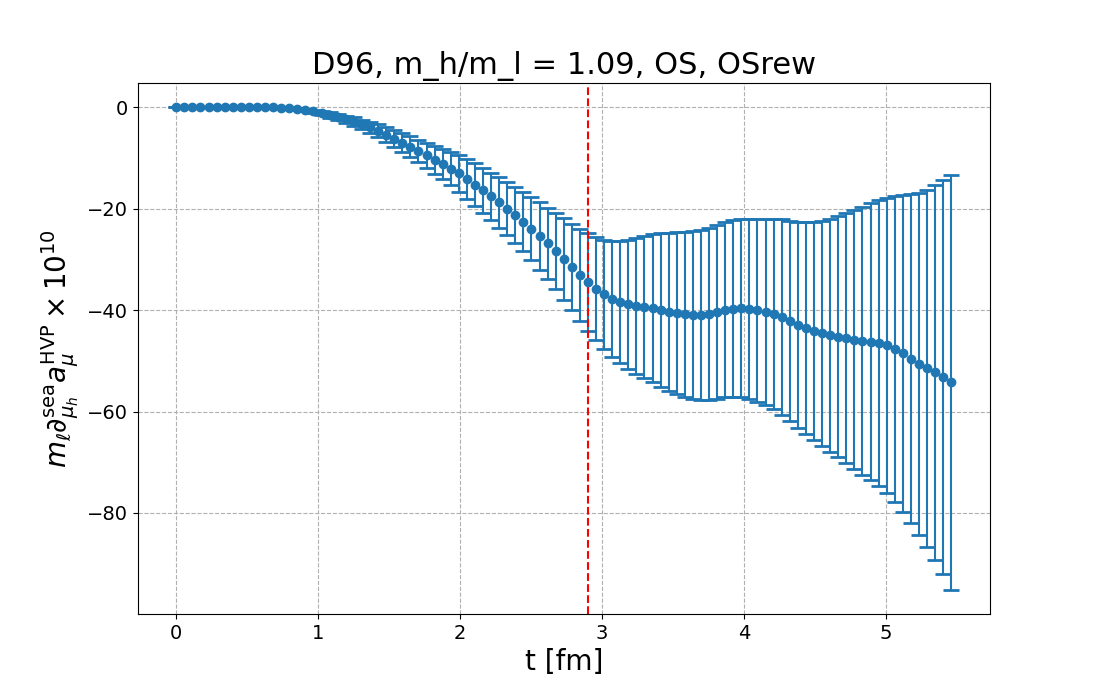
\includegraphics[trim=0cm 0.3cm 0cm 1.2cm, clip,width=\textwidth]{plots/der_mq_sea_lore/amu_D96_OS_der_001ml.png}
    \end{column}
   \end{columns}
   \

   \

   \

   \
\end{frame}
\begin{frame}
 Heavier quarks contributions: we fit a plateau in $a_\mu$ vs $t_c$ where we can see a signal. (sorry for the color choice)
    \begin{columns}
    \begin{column}{0.5\textwidth}
     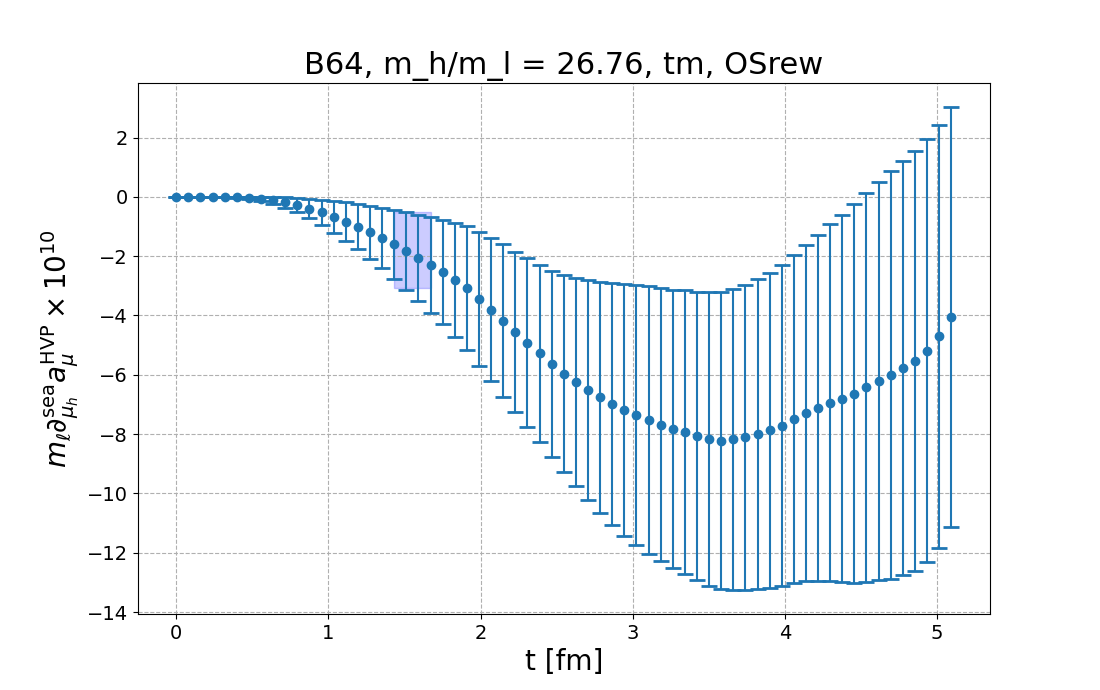
\includegraphics[trim=0cm 0.3cm 0cm 1.2cm, clip,width=\textwidth]{plots/der_mq_sea_lore/amu_B64_tm_der_026ml.png}
     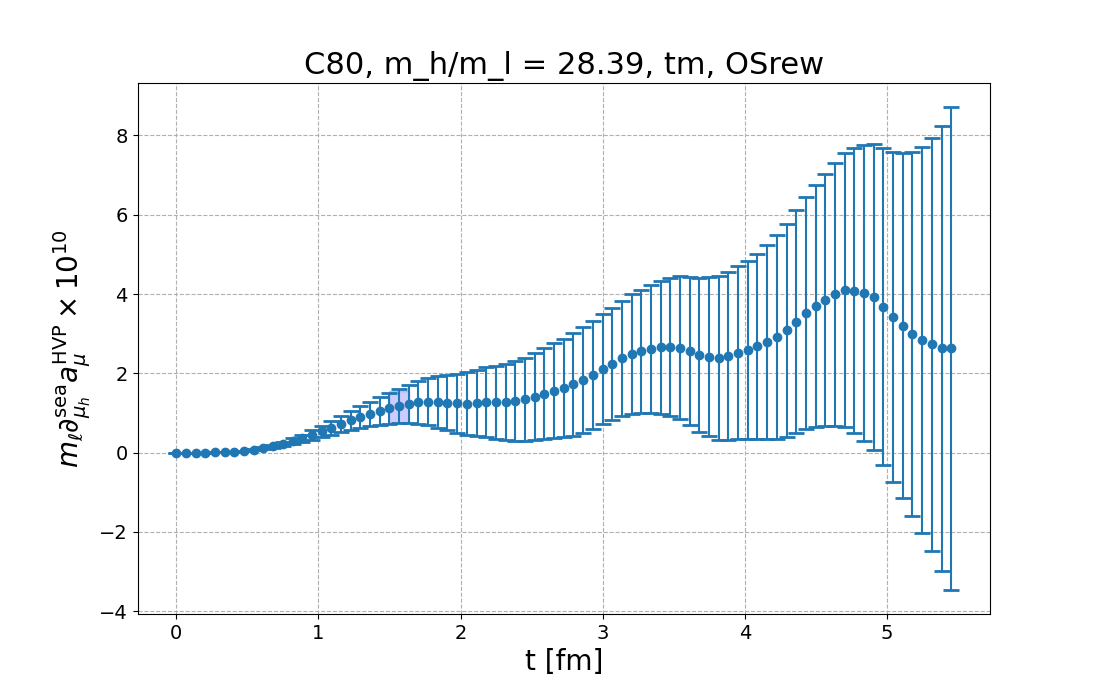
\includegraphics[trim=0cm 0.3cm 0cm 1.2cm, clip,width=\textwidth]{plots/der_mq_sea_lore/amu_C80_tm_der_028ml.png}
    \end{column}
    \begin{column}{0.5\textwidth}
     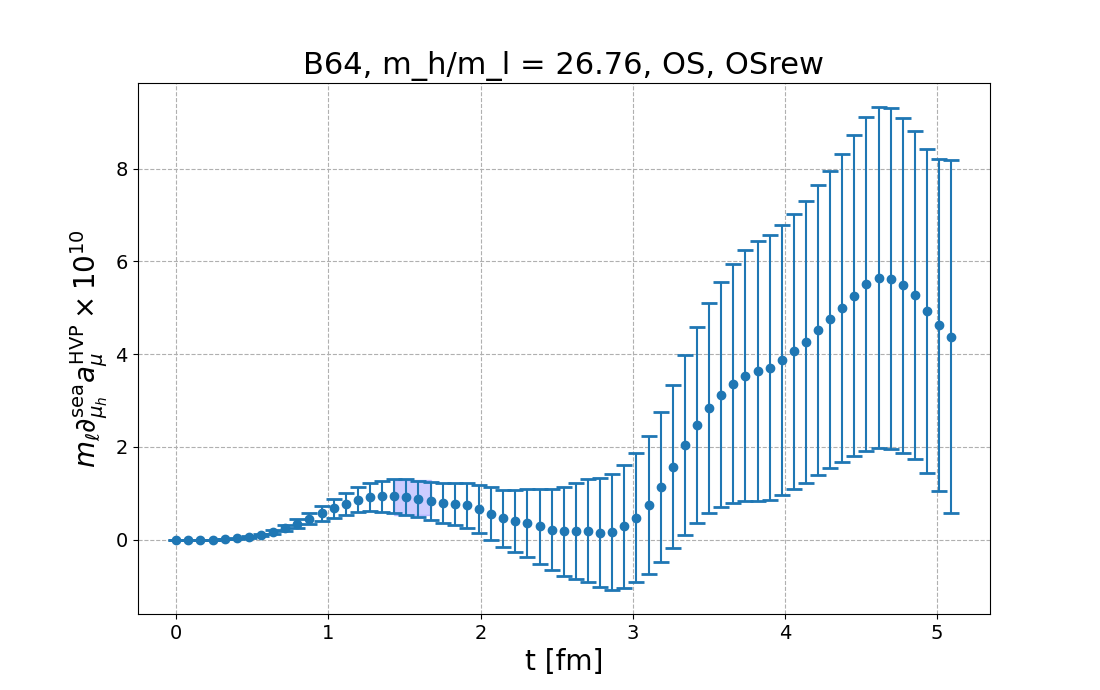
\includegraphics[trim=0cm 0.3cm 0cm 1.2cm, clip,width=\textwidth]{plots/der_mq_sea_lore/amu_B64_OS_der_026ml.png}
     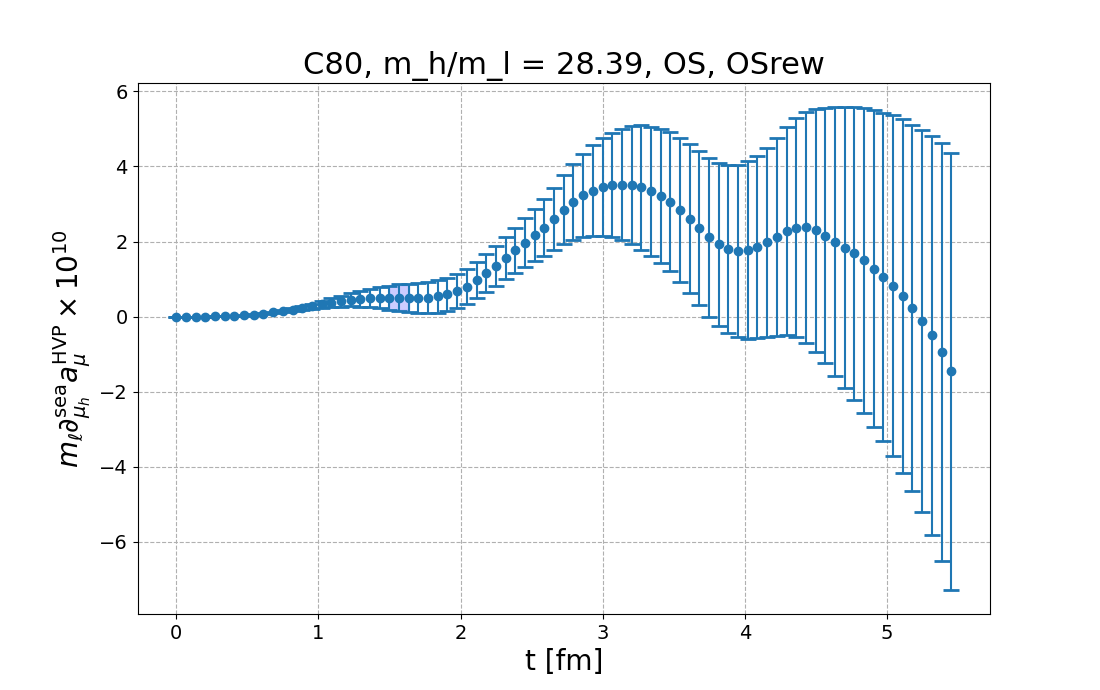
\includegraphics[trim=0cm 0.3cm 0cm 1.2cm, clip,width=\textwidth]{plots/der_mq_sea_lore/amu_C80_OS_der_028ml.png}
    \end{column}
   \end{columns}
\end{frame}
\begin{frame}
 Heavier quarks contributions: we fit a plateau in $a_\mu$ vs $t_c$ where we can see a signal. (sorry for the color choice)\vfill \,

    \

    \
    
    \
    
    \begin{columns}
    \begin{column}{0.5\textwidth}
     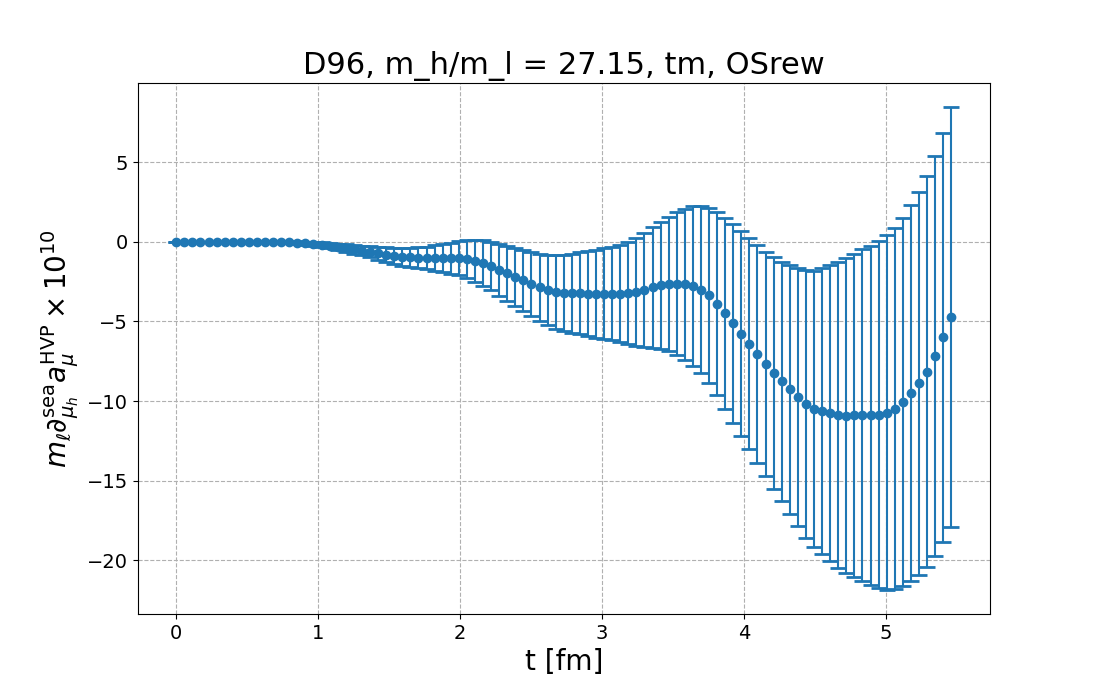
\includegraphics[trim=0cm 0.3cm 0cm 1.2cm, clip,width=\textwidth]{plots/der_mq_sea_lore/amu_D96_tm_der_027ml.png}
    \end{column}
    \begin{column}{0.5\textwidth}
     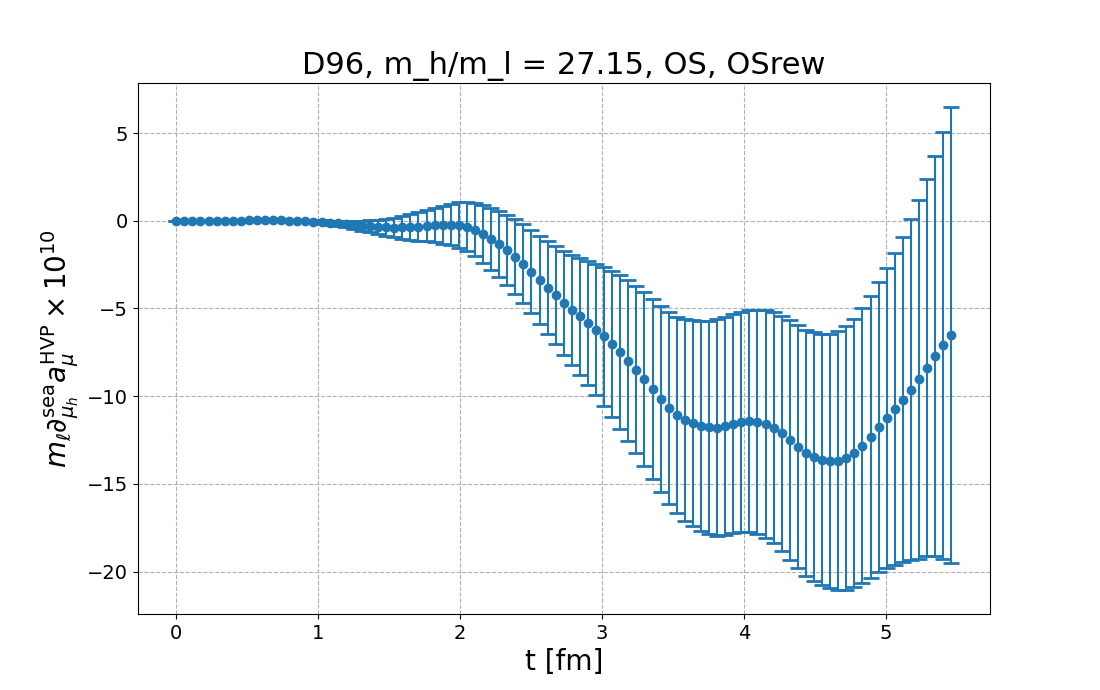
\includegraphics[trim=0cm 0.3cm 0cm 1.2cm, clip,width=\textwidth]{plots/der_mq_sea_lore/amu_D96_OS_der_027ml.png}
    \end{column}
   \end{columns}
   \

   \

   \

   \
\end{frame}
\begin{frame}
\centering
    For the $\ell$- and $s$-contributions, we performed a constant fit
    
    \
    
    \begin{columns}
        \begin{column}{0.5\textwidth}
     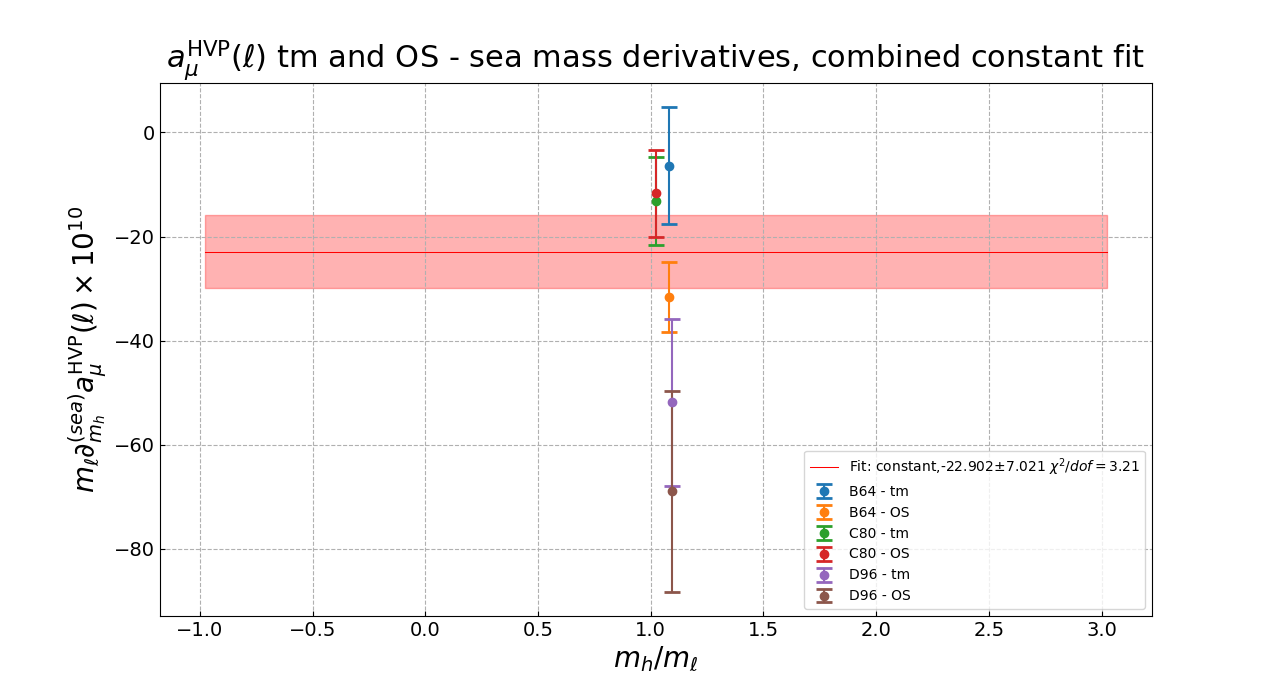
\includegraphics[trim=0cm 0.3cm 0cm 1.2cm, clip,width=\textwidth]{plots/der_mq_sea_lore/fit_amu_der_ml_full.png}

        $$\mu_\ell\times\partial^\mathrm{sea}_{\mu_\ell}a^\mathrm{HVP}_\mu(\ell)^\mathrm{conn}\times10^{10} = -22.9(7.0)$$
        
        $$\chi^2_\mathrm{red}=3.2$$
        \end{column}
        \begin{column}{0.5\textwidth}
     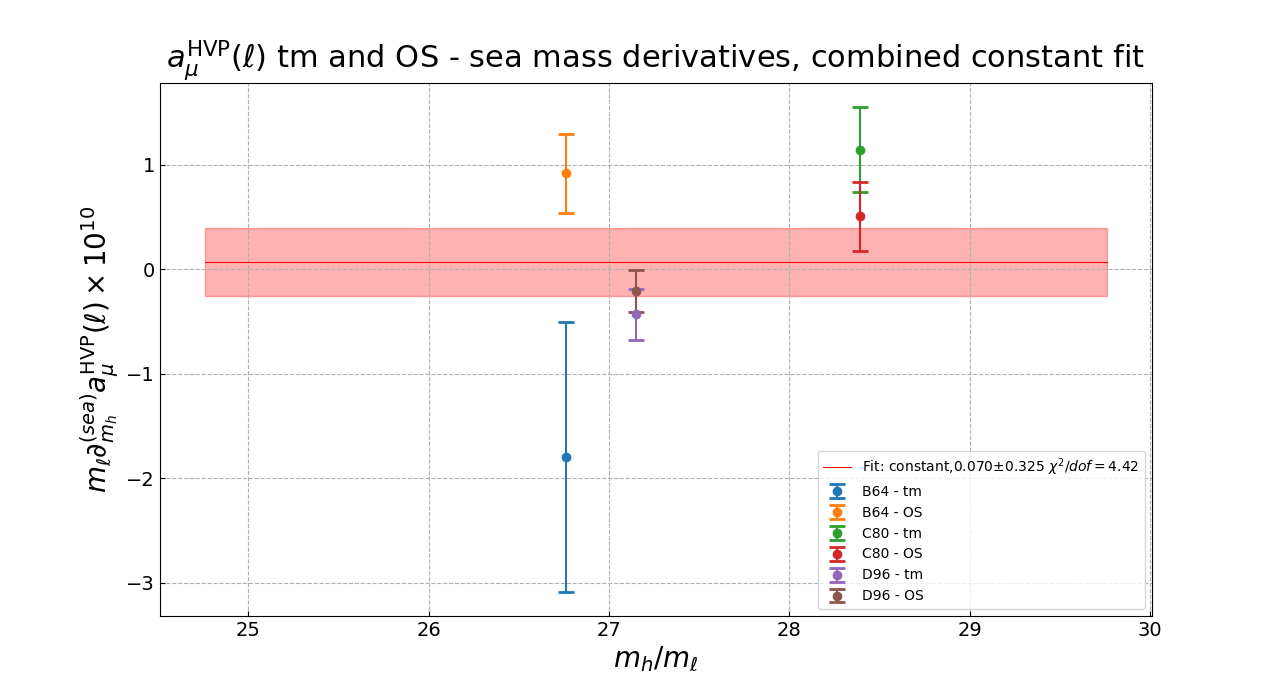
\includegraphics[trim=0cm 0.3cm 0cm 1.2cm, clip,width=\textwidth]{plots/der_mq_sea_lore/fit_amu_der_ms_full.png}
        $$\mu_\ell\times\partial^\mathrm{sea}_{\mu_s}a^\mathrm{HVP}_\mu(\ell)^\mathrm{conn}\times10^{10} = 0.070(325)$$
        
        $$\chi^2_\mathrm{red}=4.4$$
        \end{column}
    \end{columns}
    All the errors have already been rescaled with $\sqrt{\chi^2_\mathrm{red}}$
\end{frame}
\begin{frame}
\centering
    For the $c$-contribution, we performed a decoupling-inspired fit with the ansatz
    \[
   \mu_\ell  \frac{\partial a_\mu^\mathrm{HVP}(\ell)^\mathrm{conn} }{\partial\mu} = P_0\frac{1}{\mu^2}+P_1\frac{1}{\mu^2},
    \]
    
    \
    
     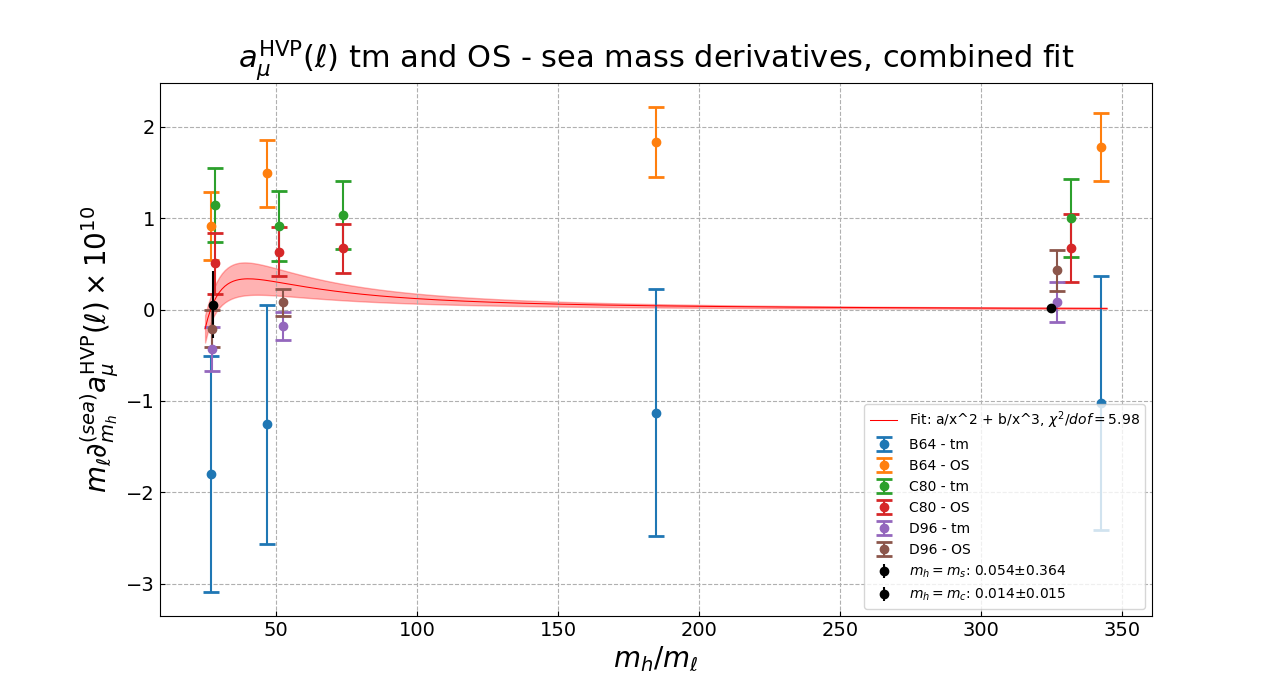
\includegraphics[trim=0cm 0.3cm 0cm 1.2cm, clip,width=0.6\textwidth]{plots/der_mq_sea_lore/fit_amu_der_mc_full.png}

        $$\mu_\ell\times\partial^\mathrm{sea}_{\mu_c}a^\mathrm{HVP}_\mu(\ell)^\mathrm{conn}\times10^{10} = 0.014(15)$$
        
        $$\chi^2_\mathrm{red}=5.98$$

        \
        
    All the errors have already been rescaled with $\sqrt{\chi^2_\mathrm{red}}$
\end{frame}
\begin{frame}
    Summarizing, the computed derivatives are

    \
    
    \begin{flalign*}
    \mu_\ell\times\partial^\mathrm{sea}_{\mu_\ell}a^\mathrm{HVP}_\mu(\ell)^\mathrm{conn}\times10^{10}& = -22.9(7.0),\\
    \mu_\ell\times\partial^\mathrm{sea}_{\mu_s}a^\mathrm{HVP}_\mu(\ell)^\mathrm{conn}\times10^{10}& = 0.070(325),\\
    \mu_\ell\times\partial^\mathrm{sea}_{\mu_c}a^\mathrm{HVP}_\mu(\ell)^\mathrm{conn}\times10^{10}& = 0.014(15).
    \end{flalign*}

    \

    \
    
    from which one can compute the shifts on the observable, listed in the table.

    \
    \begin{center}
        \begin{tabular}{c|c|c|c|c|c|c}
 & $\Delta^\mathrm{sea}_{\mu_l}$ & $\sigma(\Delta^\mathrm{sea}_{\mu_l})$& $\Delta^\mathrm{sea}_{\mu_s}$ & $\sigma(\Delta^\mathrm{sea}_{\mu_s})$ & $\Delta^\mathrm{sea}_{\mu_c}$ & $\sigma (\Delta^\mathrm{sea}_{\mu_c})$\\
\hline
\texttt{B64} &1.8235 & 0.5590 & 0.0443 & 0.2051  & 0.0632 &0.0694\\
\hline         
\texttt{C80} &0.5312 & 0.1628 & -0.0712	& 0.3295 & 0.0865 &0.0951\\
\hline         
\texttt{D96} &2.1630 & 0.6631 & 0.0232	& 0.1073  & -0.0987 &0.1085 \\
\hline         
\texttt{E112}&0.4999 & 0.1533 & -0.0473	& 0.2191  & -0.0473 &0.0520 \\
\hline
\end{tabular}
    \end{center}
\end{frame}
\end{document}
